%\ifx\wholebook\relax\else
%\documentclass[twoside]{book}
%\usepackage[active]{srcltx}
%\usepackage[LY1]{fontenc}
%\usepackage{url}
\makeatletter
\def\url@leostyle{%
  \@ifundefined{selectfont}{\def\UrlFont{\sf}}{\def\UrlFont{\sffamily}}}
\makeatother
% Now actually use the newly defined style.
\urlstyle{leo}

\usepackage{graphicx}
\def\etc{{\textit{etc}}}
\def\eg{{\textit{e.g.}}}
\def\ie{{\textit{i.e.}}}
\def\cf{{\textit{c.f.}}\ }
\def\erf{\mathop{\textrm{erf}}}
\def\sign{\mathop{\textrm{sign}}}
\def\prob{\mathop{\textrm{Prob}}}
\def\var{\mathop{\textrm{var}}}
\def\mod{\mathop{\textrm{mod}}}
\def\cor{\mathop{\textrm{cor}}}
\def\cov{\mathop{\textrm{cov}}}
\def\cl{\mathop{\textrm{CL}}}
\def\kg{\mathop{\textrm{Kg}}}
\def\patstyle#1{{\textsc #1}}
\def\th{^{\mathop{\textrm{th}}}}
%\def\st#1{^{\mathop{\rm #1}}}
\def\note#1{\begin{quote}{\textbf{Note:}} #1\end{quote}}
\def\braket#1{\left\langle #1\right\rangle}
\def\order#1{\let\o=#1$\mathcal{O}$\ifx\o 1$\left(n\right)$\else$\left(n^{#1}\right)$\fi}
%\newtheorem{privListing}{Listing}[chapter]
%\newenvironment{listing}{\vskip 3ex\hrule\vskip 1ex\begin{privListing}}{\end{privListing}\hrule\vskip 1ex}
\newtheorem{privExample}{Code example}[chapter]
\newenvironment{codeExample}{\begin{privExample}\begin{quote}\tt}{\end{quote}\end{privExample}}
\def\relboxl#1#2{\hbox to #1\hsize{#2\hfil}}
\def\relboxc#1#2{\hbox to #1\hsize{\hfil #2\hfil}}
\def\relboxr#1#2{\hbox to #1\hsize{\hfil #2}}
\def\transpose#1{\textbf{#1}^{\mathop\textrm{T}}}
\def\inverse#1{\textbf{#1}^{-1}}
%\def\tm{$^{\mathop{\rm TM}}$}
\def\tm{ }
\newenvironment{mainEquation}{\marginpar[\vspace{3 ex} Main
equation$\Rightarrow$]{\vspace{3 ex}$\Leftarrow$Main
equation}\begin{equation}}{\end{equation}}
\def\rubrique#1{\paragraph{#1}\hfil\par\noindent}

%\begin{document}
%\fi

\chapter{Optimization}
\label{ch:minimization} \vspace{1 ex}
\begin{flushright}
{\textsl Cours vite au but, mais gare \`a la chute.}\footnote{Run fast
to the goal, but beware of the fall.}\\ Alexandre Soljenitsyne
\end{flushright}
\vspace{1 ex} An optimization problem is a numerical problem where
the solution is characterized by the largest or smallest value of
a numerical function depending on several parameters. Such
function is often called the goal function. Many kinds of problems
can be expressed into optimization, that is, finding the maximum
or the minimum of a goal function. This technique has been applied
to a wide variety of fields going from operation research to game
playing or artificial intelligence. In chapter \ref{ch:estimation}
for example, the solution of maximum likelihood or least square
fits was obtained by finding the maximum, respectively the minimum
of a function.

In fact generations of high energy physicists have used the
general purpose minimization program MINUIT\footnote{F.James, M.
Roos, {\textsl MINUIT --- a system for function minimization and
analysis of the parameter errors and corrections}, Comput. Phys.
Commun., 10 (1975) 343-367.} written by Fred James\footnote{I take
this opportunity to thank Fred for the many useful discussions we
have had on the subject of minimization.} of CERN to perform least
square fits and maximum likelihood fits.  To achieve generality,
MINUIT uses several strategies to reach a minimum. In this chapter
we shall discuss a few techniques and conclude with a program
quite similar in spirit to MINUIT. Our version, however, will not
have all the features offered by MINUIT.

If the goal function can be expressed with an analytical form, the
problem of optimization can be reduced into calculating the
derivatives of the goal function respective to all parameters, a
tedious but manageable job. In most cases, however, the goal
function cannot always be expressed analytically.

Figure \ref{fig:soptimizingclasses} shows the Smalltalk class diagram.
\begin{figure}
\centering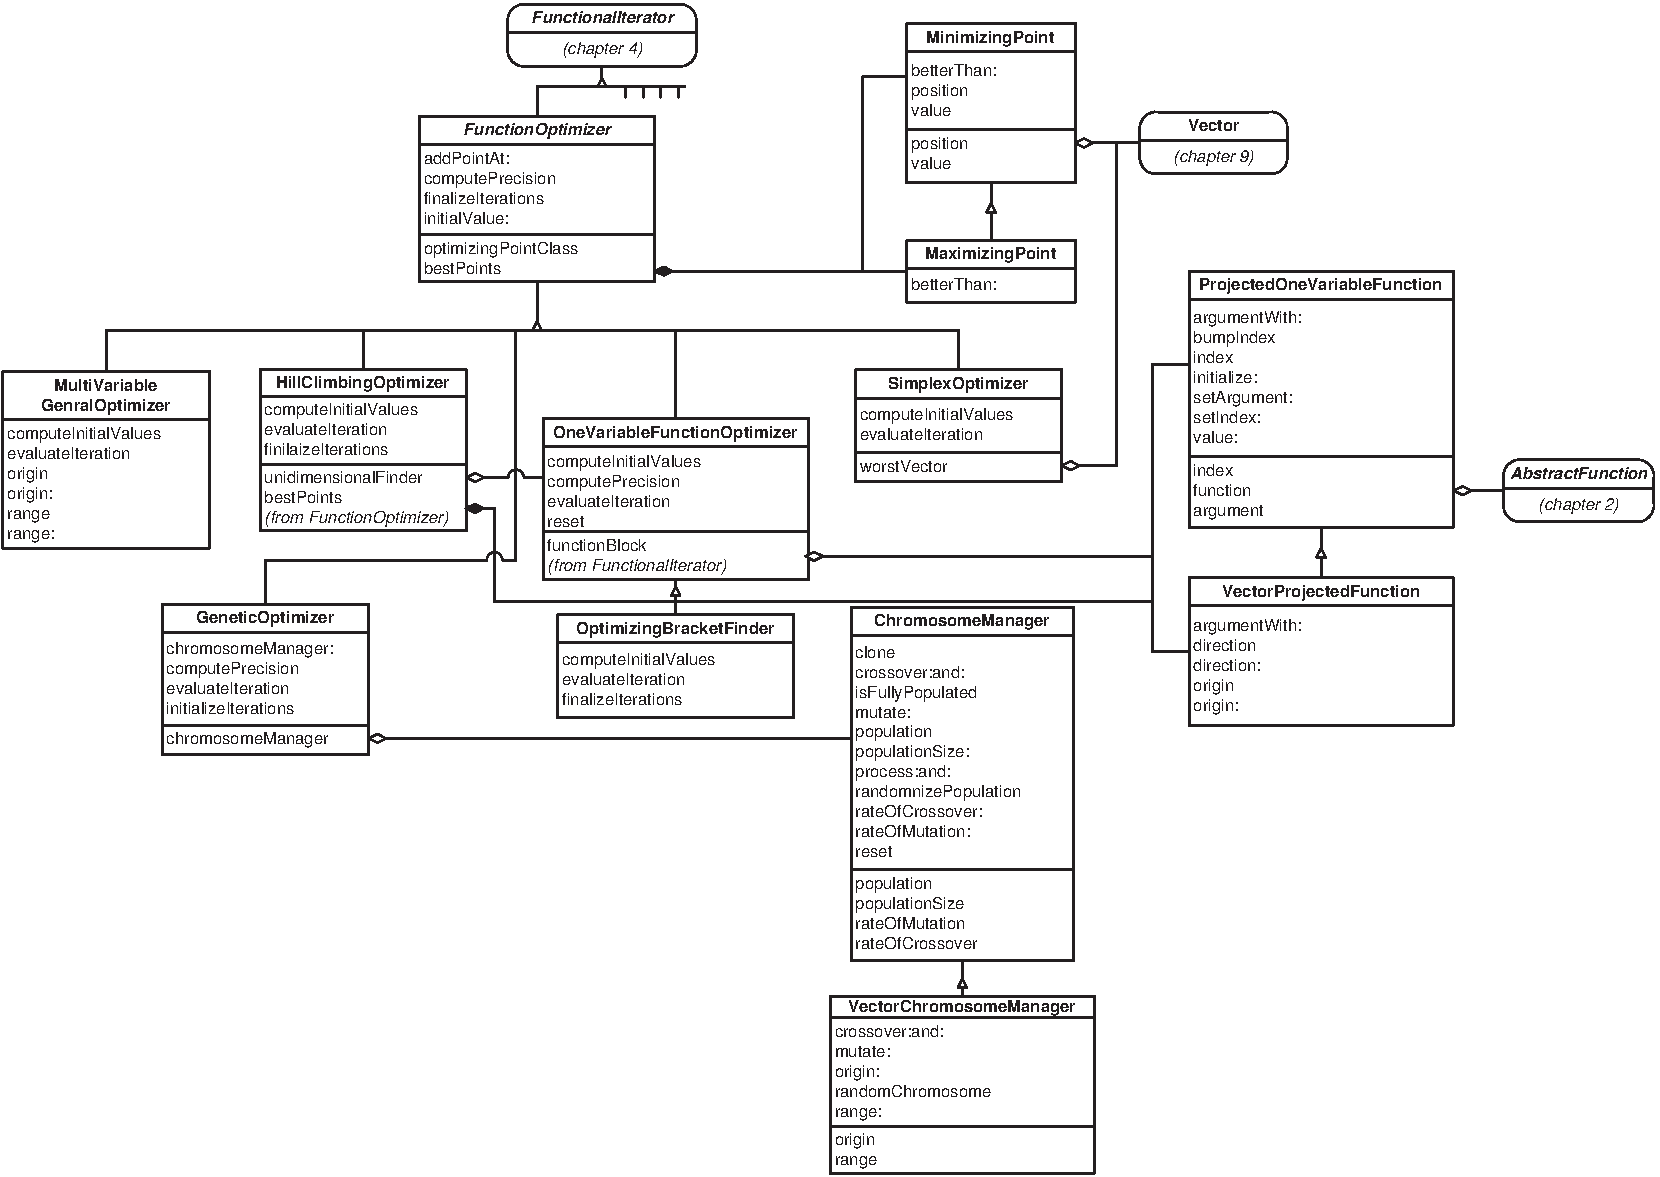
\includegraphics[width=11cm]{Figures/Optimizing}
\caption{Smalltak classes used in optimization}
\label{fig:soptimizingclasses}
\end{figure}

\section{Introduction}
\label{sec:optimum} Let us state the problem is general term. Let
$f\left({\textbf x}\right)$ be a function of a vector ${\textbf x}$ of
dimension $n$. The $n$-dimensional space is called the search
space of the problem. Depending on the problem the space can be
continuous or not. In this section we shall assume that the space
is continuous.

If the function is derivable, the gradient of the function
respective to the vector ${\textbf x}$ must vanish at the optimum.
Finding the optimum of the function can be replaced by the problem
of finding the vector ${\textbf x}$ such that:
\begin{equation}
\label{eq:mincondition}
  {d f\left({\textbf x}\right) \over d{\textbf x}} = 0.
\end{equation}
Unfortunately, the above equation is not a necessary condition for
an optimum. It can be either a maximum. a minimum or a saddle
point, that is a point where the function has a minimum in one
projection and a maximum in another projection. Furthermore, the
function may have several optima. Figure \ref{fig:localabsobulte}
shows an example of a function having two minima.
\begin{figure}
\centering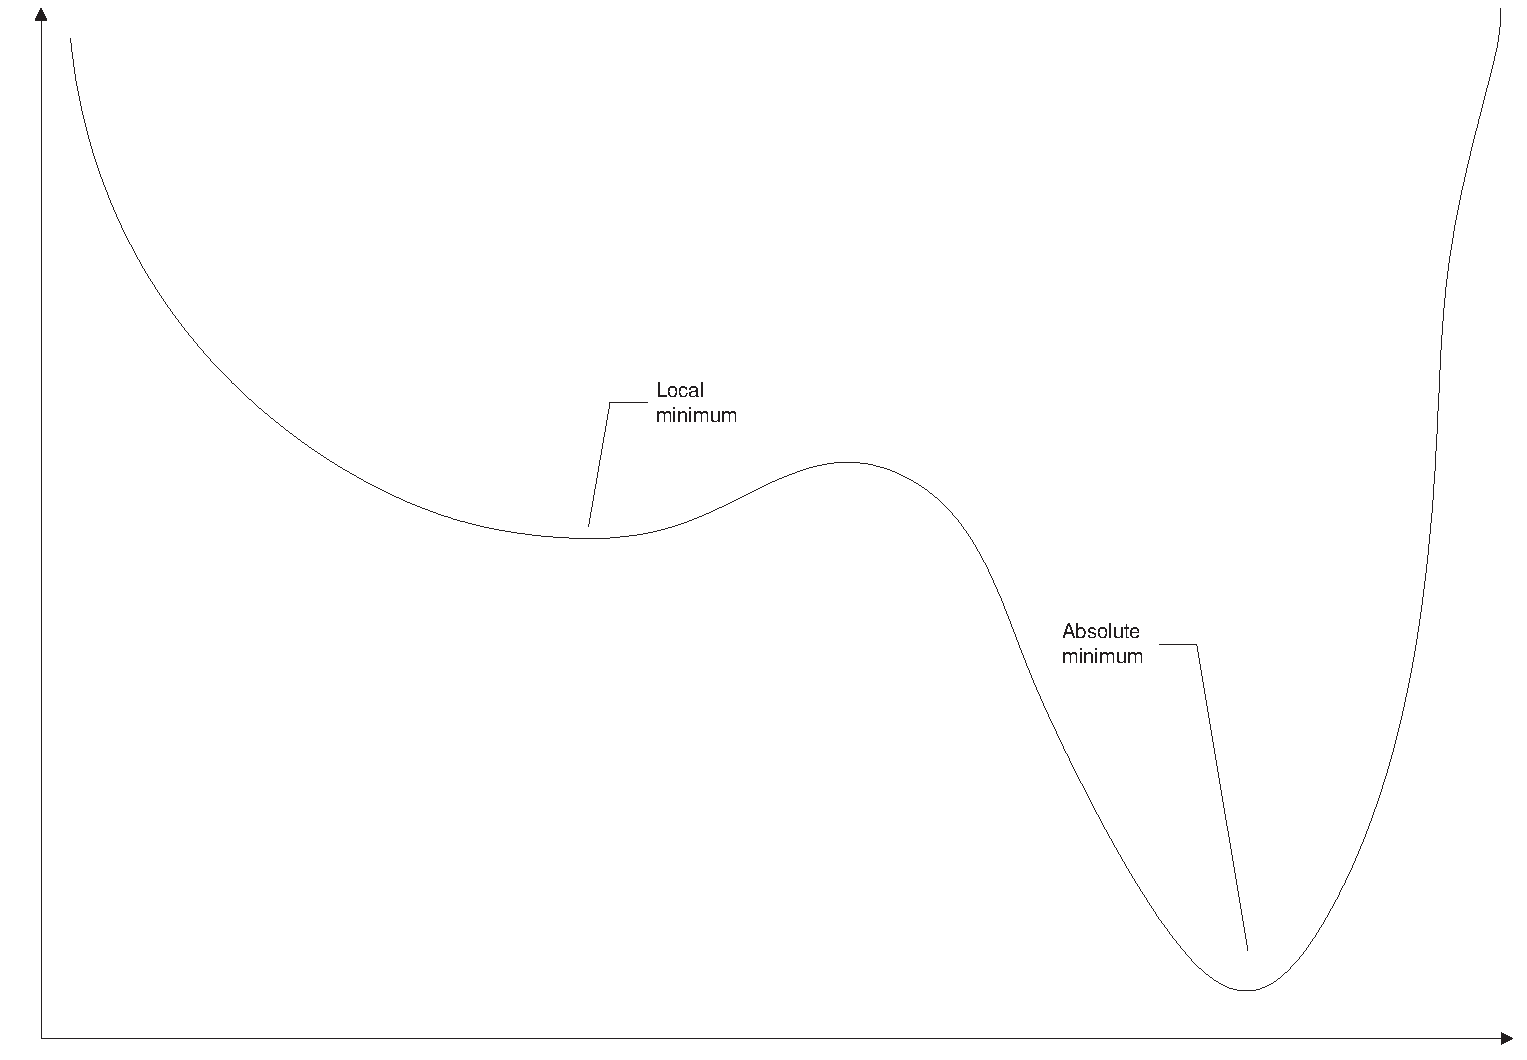
\includegraphics[width=11cm]{Figures/MinimumAbsLoc}
\caption{Local and absolute optima} \label{fig:localabsobulte}
\end{figure}
Some problems require to find the absolute optimum of the
function. Thus, one must verify that the solution of
\ref{eq:mincondition} corresponds indeed to an optimum with the
expected properties.
The reader can already see at this point that
searching for an optimum in the general case is a very difficult
task.

\noindent All optimization algorithms can be classified in two
broad categories:
\begin{itemize}
  \item {\textsl Greedy algorithms}: these algorithms are characterized by a
  local search in the most promising direction. They are usually efficient
  and quite good at finding local optima. Among greedy algorithms,
  one must distinguish those requiring the evaluation of the
  function's derivatives.
  \item {\textsl Random based algorithms}: these algorithms are using
  a random approach. They are not efficient; however, they are good at
  finding absolute optima. Simulated annealing \cite{Press} and
  genetic algorithms\cite{BerLin} belong to this class.
\end{itemize}
The table \ref{tb:optimizingalgorithms} lists the properties of
the algorithms presented in this chapter.
\begin{table}[h]
  \centering
  \caption{Optimizing algorithms presented in this book}\label{tb:optimizingalgorithms}
\vspace{1 ex}\begin{tabular}{| l | c | c |} \hline
  \hfil{\textbf Name} & {\textbf Category} & {\textbf Derivatives} \\ \hline
  Extended Newton & greedy & yes \\
  Powell's hill climbing & greedy & no \\
  Simplex & greedy & no \\
  Genetic algorithm & random based & no \\ \hline
\end{tabular}
\end{table}

\section{Extended Newton algorithms}
Extended Newton algorithms are using a generalized version of
Newton's zero finding algorithm.
These algorithms assume that the function is continuous and has only one optimum in the region
where the search is initiated.

Let us expand the function $f\left({\textbf x}\right)$ around a point
${\textbf x}^{\left(0\right)}$ near the solution.
We have in components:
\begin{equation}
  f\left({\textbf x}\right) = f\left[{\textbf x}^{\left(0\right)}\right] +\sum_j
  \left.{\partial f\left({\textbf x}\right) \over \partial x_j}\right|_{{\textbf x}={\textbf
  x}^{\left(0\right)}}
  \left[x_j-x^{\left(0\right)}_j\right].
\end{equation}
Using the expansion above into equation \ref{eq:mincondition}
yields:
\begin{equation}
\sum_j
  \left.{\partial^2 f\left({\textbf x}\right) \over \partial x_i\partial x_j}\right|_{{\textbf x}={\textbf
  x}^{\left(0\right)}}
  \left[x_j-x^{\left(0\right)}_j\right]
  + \left.{\partial f\left({\textbf x}\right) \over \partial x_i}\right|_{{\textbf x}={\textbf
  x}^{\left(0\right)}} =0.
\end{equation}
This equation can be written as a system of linear equations of
the form
\begin{equation}
  {\textbf M}\Delta = {\textbf c},
\end{equation}
where $\Delta_j =x_j-x^{\left(0\right)}_j$. The components of the
matrix ${\textbf M}$ --- called the Hessian matrix --- are given by:
\begin{equation}
  m_{ij} = \left.{\partial^2 f\left({\textbf x}\right) \over \partial x_i\partial x_j}\right|_{{\textbf x}={\textbf
  x}^{\left(0\right)}},
\end{equation}
and the components of the vector ${\textbf c}$ are given by:
\begin{equation}
  c_i = -\left.{\partial f\left({\textbf x}\right) \over \partial x_i}\right|_{{\textbf x}={\textbf
  x}^{\left(0\right)}}.
\end{equation}
Like in section \ref{sec:lsfnonlin} one can iterate this process
by replacing ${\textbf x}^{\left(0\right)}$ with ${\textbf
x}^{\left(0\right)}+\Delta$. This process is actually equivalent
to the Newton zero finding method (\cf section \ref{sec:newton}).
The final solution is a minimum if the matrix ${\textbf M}$ is
positive definite; else it is a maximum.

This technique is used by MINUIT in the vicinity of the goal
function's optimum. It is the region where the algorithm described
above works well. Far from the optimum, the risk of reaching a
point where the matrix ${\textbf M}$ cannot be inverted is quite high
in general. In addition, the extended Newton algorithm requires
that the second order derivatives of the function can be computed
analytically; at least the first order derivatives must be
provided, otherwise the cost of computation at each step becomes
prohibitive. A concrete implementation of the technique is not
given here. The reader can find in this book all the necessary
tools to make such an implementation. It is left as a exercise for
the reader. In the rest of this chapter, we shall present other
methods which work without an analytical knowledge of the
function.

\section{Hill climbing algorithms}
Hill climbing is a generic term covering many algorithms trying to
reach an optimum by determining the optimum along successive
directions. The general algorithm is outlined below.
\begin{enumerate}
  \item select an initial point ${\textbf x}_0$ and a direction ${\textbf v}$;
  \item find ${\textbf x}_1$, the optimum of the function along the selected
  direction;
  \item if convergence is attained, terminate the algorithm;
  \item set ${\textbf x}_0={\textbf x}_1$, select a different direction and go back to step 2.
\end{enumerate}
The simplest of these algorithms simply follows each axis in turn
until a convergence is reached. More elaborate algorithms
exist\cite{Press}. One of them is described in section
\ref{sec:powell}.

Hill climbing algorithms can be applied to any continuous
function, especially when the function's derivatives are not
easily calculated. The core of the hill climbing algorithm is
finding the optimum along one direction. Let ${\textbf v}$ be the
direction, then finding the optimum of the vector function
$f\left({\textbf x}\right)$ along the direction ${\textbf v}$ starting
from point ${\textbf x}_0$ is equivalent to finding the optimum of the
one-variable function $g\left(\lambda\right)=f\left({\textbf
x}_0+\lambda{\textbf v}\right)$.

Therefore, in order to implement a hill climbing algorithm, we
first need to implement an algorithm able to find the optimum of a
one-variable function. This is the topic of the sections
\ref{sec:optonedim} and \ref{sec:bracket}. Before this, we need to
discuss the implementation details providing a common framework to
all classes discussed in the rest of this chapter.

\subsection{Optimizing --- General implementation}
\label{sec:goptonedim} At this point the reader may be a little
puzzled by the use of {\textsl optimum} instead of speaking of minimum
or maximum. We shall now disclose a general implementation which
works both for finding a minimum or a maximum. This should not
come to a surprise since, in mathematics, a minimum or a maximum
are both very similar --- position where the derivative of a
function vanishes
--- and can be easily turned into each other --- e.g. by negating the
function.

To implement a general purpose optimizing framework, we introduce
two new classes: {\texttt MinimizingPoint} and {\texttt MaximizingPoint},
 a subclass of {\texttt MinimizingPoint}. These two classes
are used as \patstyle{Strategy} by the optimizing algorithms. The
class {\texttt MinimizingPoint} has two instance variables
\begin{description}
  \item[\texttt value] the value of the goal function, that is
  $g\left(\lambda\right)$ or $f\left({\textbf x}\right)$;
  \item[\texttt position] the position at which the function has been
  evaluated, that is $\lambda$ or ${\textbf x}$.
\end{description}
The class {\texttt MinimizingPoint} contains most of the methods. The
only method overloaded by the class {\texttt MaximizingPoint} is the
method {\texttt betterThan}, which tells whether an optimizing point
is better than another. The method {\texttt betterThan} can be used in
all parts of the optimizing algorithms to find out which point is
the optimum so far. In algorithms working in multiple dimensions,
the method {\texttt betterThan} is also used to sort the points from
the best to the worst.

A convenience instance creation method allows to create instances
for a given function with a given argument. The instance is then
initialized with the function's value evaluated at the argument.
Thus, all optimizing algorithms described here do not call the
goal function explicitly.

Otherwise the implementation of the one dimensional optimum search
uses the general framework of the iterative process. More
specifically it uses the class {\texttt FunctionalIterator} described
in section \ref{sec:iterrel}.

A final remark concerns the method {\texttt initializeIteration}. The
golden search algorithm assume that the 3 points $\lambda_0$,
$\lambda_1$ and $\lambda_2$ have been determined. What if they
have not been? In this case, the method {\texttt initializeIteration}
uses the optimum bracket finder described in section
\ref{sec:bracket}

\subsection{Common optimizing classes}
%\label{sec:sgeneralOpt} \marginpar{Figure
%\ref{fig:soptimizingclasses} with the boxes {\textbf
%FunctionOptimizer}, {\textbf MinimizingPoint}, {\textbf MaximizingPoint},
%{\textbf ProjectedOneVariableFunction} and {\textbf
%  VectorProjectedFunction} grayed.}

In Pharo we have two classes of optimizing points: {\texttt PMMinimizingPoint}
and its subclass {\texttt PMMaximizingPoint}.
These classes are shown in listing
\ref{ls:optimizerCommon}.
The class {\texttt PMFunctionOptimizer} is
in charge of handling the management of the optimizing points.
This clas is shown in listing \ref{ls:optimizerAbstract}.

\noindent The class {\texttt PMMinimizingPoint} has the following
instance variables:
\begin{description}
  \item[\texttt position] contains the position at which the function
  is evaluated; this instance variable is a number if the function
  to optimize is a one variable function and an array or a vector
  if the function to evaluate is a function of many variables;
  \item[\texttt value] contains the value of the function evaluated at the point's position;
\end{description}
Accessor methods corresponding to these variables are supplied. As
we noted in section \ref{sec:goptonedim}, the only method
redefined by the subclass {\texttt PMMaximizingPoint} is the method
{\texttt betterThan:} used to decide whether a point is better than
another.

Optimizing points are created with the convenience method {\texttt
vector:function:} which evaluates the function supplied as second
argument at the position supplied as the first argument.

\begin{listing}[label=ls:optimizerCommon]{Smalltalk}
{Smalltalk classes common to all optimizing classes}
Object subclass: #PMMinimizingPoint
   instanceVariableNames: 'value position'
   classVariableNames: ''
   package: 'Math-Numerical-Math-FunctionIterator'
\end{listing}

\begin{displaycode}{Smalltalk}
PMMinimizingPoint class>>new: aVector value: aNumber
   ^ self new vector: aVector; value: aNumber; yourself  
\end{displaycode}  

\begin{displaycode}{Smalltalk}
PMMinimizingPoint class>>vector: aVector function: aFunction
   ^ self new: aVector value: (aFunction value: aVector)
\end{displaycode}

\begin{displaycode}{Smalltalk}
PMMinimizingPoint>>betterThan: anOptimizingPoint
   ^ value < anOptimizingPoint value
\end{displaycode}

\begin{displaycode}{Smalltalk}
PMMinimizingPoint>>position
   ^ position
\end{displaycode}

\begin{displaycode}{Smalltalk}
PMMinimizingPoint>>printOn: aStream
   position printOn: aStream.
   aStream
      nextPut: $:;
      space.
      value printOn: aStream
\end{displaycode}        
%$

\begin{displaycode}{Smalltalk}
PMMinimizingPoint>>value
   ^ value
\end{displaycode}

\begin{displaycode}{Smalltalk}
PMMinimizingPoint>>value: aNumber
   value := aNumber.
\end{displaycode}

\begin{displaycode}{Smalltalk}
PMMinimizingPoint>>vector: aVector
    position := aVector
\end{displaycode}

\begin{displaycode}{Smalltalk}
PMMinimizingPoint subclass: #PMMaximizingPoint
   instanceVariableNames: ''
   classVariableNames: ''
   package: 'Math-Numerical-Math-FunctionIterator'
\end{displaycode}

\begin{displaycode}{Smalltalk}
PMMaximizingPoint>>betterThan: anOptimizingPoint
   ^ value > anOptimizingPoint value
\end{displaycode}
 
The class {\texttt PMFunctionOptimizer} is in charge of handling the
optimizing points. it has the following instance variables:
\begin{description}
  \item[\texttt optimizingPointClass] is the class of the optimizing
  points used as \patstyle{Strategy} by the optimizer; it is used
  to create instances of points at a given position for a given
  function;
  \item[\texttt bestPoints] contains a sorted collection of optimizing
  points; the best point is the first and the worst point is the
  last; all optimizers rely on the fact that sorting is done by this sorted collection.
\end{description}
The method {\texttt addPointAt:} creates an optimizing point at the
position supplied as argument and adds this point to the
collection of best points. Since that collection is sorted, one is
always certain to find the best result in the first position. This
fact is used by the method {\texttt finalizeIterations}, which
retrieves the result from the collection of best points.

Instances of the function optimizer are created with the two
convenience methods {\texttt minimizingFuntion:} and {\texttt
maximizingFuntion:} helping to define the type of optimum. An
additional convenience method, {\texttt forOptimizer:} allows to
create a new optimizer with the same strategy --- that is, the
same class of optimizing points --- and the same function as the
optimizer supplied as argument.
This method is used to create optimizers used in intermediate steps.

Because finding an optimum cannot be determined numerically with
high precision \cite{Press} the class {\texttt PMFunctionOptimizer}
redefines the method {\texttt defaultPrecision} to be 100 times the
default numerical precision.
\begin{listing} Smalltalk abstract class for all optimizing classes \label{ls:optimizerAbstract}
$$\halign{ #\hfil&\quad#\hfil\cr {\sl Class}& {\Large\bf DhbFunctionOptimizer}\cr
{\sl Subclass of }&{\tt DhbFunctionalIterator}\cr\noalign{\vskip 1ex}

{\sl Instance variable names:}&\parbox[t]{4 in}{\tt  optimizingPointClass bestPoints }\cr\noalign{\vskip 1ex}}$$


Class methods
{\parskip 1ex\par\noindent}
{\bf defaultPrecision}
\begin{verbatim}
    ^ super defaultPrecision * 100
\end{verbatim}
{\bf forOptimizer:} {\tt aFunctionOptimizer}
\begin{verbatim}
    ^ self new initializeForOptimizer: aFunctionOptimizer
\end{verbatim}
{\bf maximizingFunction:} {\tt aFunction}
\begin{verbatim}
    ^ super new initializeAsMaximizer; setFunction: aFunction
\end{verbatim}
{\bf minimizingFunction:} {\tt aFunction}
\begin{verbatim}
    ^ super new initializeAsMinimizer; setFunction: aFunction
\end{verbatim}



Instance methods
{\parskip 1ex\par\noindent}
{\bf addPointAt:} {\tt aNumber}
\begin{verbatim}
    bestPoints add: (optimizingPointClass vector: aNumber
                                        function: functionBlock)
\end{verbatim}
{\bf bestPoints}
\begin{verbatim}
    ^ bestPoints
\end{verbatim}
{\bf finalizeIterations}
\begin{verbatim}
    result := bestPoints first position.
\end{verbatim}
{\bf functionBlock}
\begin{verbatim}
    ^ functionBlock
\end{verbatim}
{\bf initialize}
\begin{verbatim}
    bestPoints := SortedCollection sortBlock:
                                         [ :a :b | a betterThan: b ].
    ^ super initialize
\end{verbatim}
{\bf initializeAsMaximizer}
\begin{verbatim}
    optimizingPointClass := DhbMaximizingPoint.
    ^ self initialize
\end{verbatim}
{\bf initializeAsMinimizer}
\begin{verbatim}
    optimizingPointClass := DhbMinimizingPoint.
    ^ self
\end{verbatim}
{\bf initializeForOptimizer:} {\tt aFunctionOptimizer}
\begin{verbatim}
    optimizingPointClass := aFunctionOptimizer pointClass.
    functionBlock := aFunctionOptimizer functionBlock.
    ^ self initialize
\end{verbatim}
{\bf initialValue:} {\tt aVector}
\begin{verbatim}
    result := aVector copy.
\end{verbatim}
{\bf pointClass}
\begin{verbatim}
    ^ optimizingPointClass
\end{verbatim}
{\bf printOn:} {\tt aStream}
\begin{verbatim}
    super printOn: aStream.
    bestPoints do: [ :each | aStream cr. each printOn: aStream ].
\end{verbatim}

\end{listing}

In order to find an optimum along a given direction, one needs to
construct an object able to transform a vector function into a one
variable function.
The class {\texttt PMProjectedOneVariableFunction} and its subclass {\texttt
  PMVectorProjectedFunction} provide this functionality.
They are shown in listing \ref{ls:projectedfunctions}.
The class {\texttt PMProjectedOneVariableFunction} has the following instance
variables:
\begin{description}
  \item[\texttt function] the goal function $f\left({\textbf x}\right)$;
  \item[\texttt argument] the vector argument of the goal function,
  that is the vector ${\textbf x}$;
  \item[\texttt index] the index of the axis along which the function
  is projected.
\end{description}
The instance variables {\texttt argument} and {\texttt index} can be read
and modified using direct accessor methods.
The goal function is set only at creation time: the instance creation method {\texttt
function:} take the goal function as argument.
A convenience method {\texttt bumpIndex} allows to alter the index in circular
fashion\footnote{We do not give the implementation of the simplest
of the hill climbing algorithms using alternatively each axes of
the reference system. This implementation, which uses the method
{\texttt bumpIndex}, is left as an exercise for the reader.}.

The class {\texttt PMVectorProjectedFunction} has no additional
variables. Instead it is reusing the instance variable {\texttt index}
as the direction along which the function is evaluated. For
clarity, the accessor methods have been renamed {\texttt direction},
{\texttt direction:}, {\texttt origin} and {\texttt origin:}.

For both classes, the method {\texttt argumentAt:} returns the
argument vector for the goal function, that is the vector ${\textbf
x}$. The method {\texttt value:} returns the value of the function
$g\left(\lambda\right)$ for the supplied argument $\lambda$.

\begin{listing}[label=ls:projectedfunctions]{Smalltalk}
{Smalltalk projected function classes}
Object subclass: #PMProjectedOneVariableFunction
   instanceVariableNames: 'index function argument'
   classVariableNames: ''
   package: 'Math-Numerical'
\end{listing}

\begin{displaycode}{Smalltalk}
PMProjectdOneVariableFunction class>>function: aVectorFunction
    ^ super new initialize: aVectorFunction
\end{displaycode}

\begin{displaycode}{Smalltalk}
PMProjectdOneVariableFunction>>argumentWith: aNumber
    ^ argument at: index put: aNumber; yourself
\end{displaycode}

\begin{displaycode}{Smalltalk}
PMProjectdOneVariableFunction>>bumpIndex
    index isNil
        ifTrue: [ index := 1]
        ifFalse: [ index := index + 1.
                  index > argument size
                    ifTrue: [ index := 1].
                ]
\end{displaycode}

\begin{displaycode}{Smalltalk}
PMProjectdOneVariableFunction>>index
    index isNil
        ifTrue: [ index := 1].
    ^ index
\end{displaycode}

\begin{displaycode}{Smalltalk}
PMProjectdOneVariableFunction>>initialize: aFunction
    function := aFunction.
    ^ self
\end{displaycode}

\begin{displaycode}{Smalltalk}
PMProjectdOneVariableFunction>>setArgument: anArrayOrVector
    argument := anArrayOrVector copy
\end{displaycode}

\begin{displaycode}{Smalltalk}
PMProjectdOneVariableFunction>>setIndex: anInteger
    index := anInteger
\end{displaycode}

\begin{displaycode}{Smalltalk}
PMProjectdOneVariableFunction>>value: aNumber
    ^ function value: ( self argumentWith: aNumber)
\end{displaycode}


\begin{displaycode}{Smalltalk}
PMProjectedOneVariableFunction subclass: #PMVectorProjectedFunction
   instanceVariableNames: ''
   classVariableNames: ''
   package: 'Math-Numerical'
\end{displaycode}

\begin{displaycode}{Smalltalk}
PMVectorProjectedFunction>>argumentWith: aNumber
    ^ aNumber * self direction + self origin
\end{displaycode}

\begin{displaycode}{Smalltalk}
PMVectorProjectedFunction>>direction
    ^ index
\end{displaycode}

\begin{displaycode}{Smalltalk}
PMVectorProjectedFunction>>direction: aVector
    index := aVector.
\end{displaycode}

\begin{displaycode}{Smalltalk}
PMVectorProjectedFunction>>origin}
    ^ argument
\end{displaycode}

\begin{displaycode}{Smalltalk}
PMVectorProjectedFunction>>origin: aVector
    argument := aVector
\end{displaycode}

\begin{displaycode}{Smalltalk}
PMVectorProjectedFunction>>printOn:aStream
    self origin printOn: aStream.
    aStream nextPutAll: ' ('.
    self direction printOn: aStream.
    aStream nextPut: $).
\end{displaycode}
%$
\section{Optimizing in one dimension}
\label{sec:optonedim} To find the optimum of a one-variable
function, $g\left(\lambda\right)$, whose derivative is unknown,
the most robust algorithm is an algorithm similar to the bisection
algorithm described in section \ref{sec:bisection}.

Let us assume that we have found three points $\lambda_0$,
$\lambda_1$ and $\lambda_2$ such that
$\lambda_0<\lambda_1<\lambda_2$ and such that
$g\left(\lambda_1\right)$ is better than both
$g\left(\lambda_0\right)$ and $g\left(\lambda_2\right)$. If the
function $g$ is continuous over the interval
$\left[\lambda_0,\lambda_2\right]$, then we are certain that an
optimum of the function is located in the interval
$\left[\lambda_0,\lambda_2\right]$. As for the bisection
algorithm, we shall try to find a new triplet of values with
similar properties while reducing the size of the interval. A
point is picked in the largest of the two intervals
$\left[\lambda_0,\lambda_1\right]$ or
$\left[\lambda_1,\lambda_2\right]$ and is used to reduce the
initial interval.

If $\lambda_1-\lambda_0\leq\lambda_2-\lambda_1$ we compute
$\lambda_4 =\lambda_1 + \omega\left(\lambda_2-\lambda_1\right)$
where $\omega$ is the golden
section\footnote{$\omega={3-\sqrt{5}\over 2}\approx0.38197$} from
Pythagorean lore. Choosing $\omega$ instead of $1/2$ ensures that
successive intervals have the same relative scale. A complete
derivation of this argument can be found in \cite{Press}. If
$\lambda_4$ yields a better function value than $\lambda_1$, the
new triplet of point becomes $\lambda_1$, $\lambda_4$ and
$\lambda_2$; otherwise, the triplet becomes $\lambda_0$,
$\lambda_1$ and $\lambda_4$.

If we have $\lambda_1-\lambda_0>\lambda_2-\lambda_1$ we compute
$\lambda_4 =\lambda_1 + \omega\left(\lambda_0-\lambda_1\right)$.
Then the new triplets can be either $\lambda_0$, $\lambda_4$ and
$\lambda_1$, or $\lambda_4$, $\lambda_1$ and $\lambda_2$.

The reader can verify that the interval decreases steadily
although not as fast as in the case of bisection where the
interval is halved at each iteration.
Since the algorithm is using the golden section it is called golden section search.

By construction the golden section search algorithm makes sure
that the optimum is always located between the points $\lambda_0$
and $\lambda_2$. Thus, at each iteration, the quantity
$\lambda_2-\lambda_0$ give an estimate of the error on the
position of the optimum.

\subsection{Optimizing in one dimension}
%\marginpar{Figure \ref{fig:soptimizingclasses} with the box {\textbf
%OneVariableFunctionOptimizer} grayed.}
Listing \ref{ls:optimizerOneDim} shows the class {\texttt
PMOneVariableFunctionOptimizer} implementing the search for an
optimum of a one-variable function using the golden section
search.
The following code example shows how to use this class to
find the maximum of the gamma distribution discussed in section
\ref{sec:gammadist}.

\begin{displaycode}{Smalltalk}
| distr finder maximum |
   distr := PMGammaDistribution shape: 2 scale: 5.
   finder := PMOneVariableFunctionOptimizer maximizingFunction: distr.
   maximum := finder evaluate
\end{displaycode}

The first line after the declarations creates a new instance of a
gamma distribution with parameters $\alpha = 2$ and $\beta = 5$.
The next line creates an instance of the optimum finder. The
selector used to create the instance selects a search for a
maximum. The last line is the familiar statement to evaluate the
iterations --- that is, performing the search for the maximum ---
and to retrieve the result. Since no initial value was supplied
the search begins at a random location.

The class {\texttt PMOneVariableFunctionOptimizer} is a subclass of
the class {\texttt PMFunctionOptimizer}. It does not need any additional
instance variables. The golden section is kept as a class variable
and is calculated at the first time it is needed.

At each iteration the method {\texttt nextXValue} is used to compute
the next position at which the function is evaluated. This
corresponding new optimizing point is added to the collection of
best points. Then, the method {\texttt indexOfOuterPoint} is used to
determine which point must be discarded: it is always the second
point on either side of the best point. The precision of the
result is estimated from the bracketing interval in the method
{\texttt computePrecision}, using relative precision (of course!).

The method {\texttt addPoint:} of the superclass can be used to supply
an initial bracketing interval. The method {\texttt
computeInitialValues} first checks whether a valid bracketing
interval has been supplied into the collection of best points. If
this is not the case, a search for a bracketing interval is
conducted using the class {\texttt PMOptimizingBracketFinder}
described in section \ref{sec:sbracket}. The instance of the
bracket finder is created with the method {\texttt forOptimizer:} so
that its strategy and goal function are taken over from the golden
section optimum finder.

\begin{listing}[label=ls:optimizerOneDim]{Smalltalk}
{Smalltalk golden section optimum finder}
PMFunctionOptimizer subclass: #PMOneVariableFunctionOptimizer
   instanceVariableNames: ''
   classVariableNames: 'GoldenSection'
   package: 'Math-Numerical-Math-FunctionIterator'
\end{listing}

\begin{displaycode}{Smalltalk}
PMOneVariableFunctionOptimizer class>>defaultPrecision
    ^ PMFloatingPointMachine new defaultNumericalPrecision * 10
\end{displaycode}

\begin{displaycode}{Smalltalk}
PMOneVariableFunctionOptimizer class>>goldenSection
    GoldenSection isNil ifTrue: [GoldenSection := (3 - 5 sqrt) / 2].
    ^ GoldenSection
\end{displaycode}

\begin{displaycode}{Smalltalk}
PMOneVariableFunctionOptimizer>>computeInitialValues
    [ bestPoints size  > 3 ] whileTrue: [ bestPoints removeLast ].
    bestPoints size = 3
        ifTrue: [ self hasBracketingPoints
                    ifFalse: [ bestPoints removeLast ].
                ].
    bestPoints size < 3
        ifTrue: [ (PMOptimizingBracketFinder forOptimizer: self) evaluate ].
\end{displaycode}

\begin{displaycode}{Smalltalk}
PMOneVariableFunctionOptimizer>>computePrecision
    ^ self precisionOf: ((bestPoints at: 2) position - (bestPoints 
                                                  at: 3) position) abs
           relativeTo: (bestPoints at: 1) position abs
\end{displaycode}

\begin{displaycode}{Smalltalk}
PMOneVariableFunctionOptimizer>>evaluateIteration
    self addPointAt: self nextXValue.
    bestPoints removeAtIndex: self indexOfOuterPoint.
    ^ self computePrecision
\end{displaycode}

\begin{displaycode}{Smalltalk}
PMOneVariableFunctionOptimizer>>hasBracketingPoints
    | x1 |
    x1 := (bestPoints at: 1) position.
    ^ ((bestPoints at: 2) position - x1) * ((bestPoints at: 3) 
                                                    position - x1) < 0
\end{displaycode}
                                                  
\begin{displaycode}{Smalltalk}
PMOneVariableFunctionOptimizer>>indexOfOuterPoint
    | inferior superior x |
    inferior := false.
    superior := false.
    x := bestPoints first position.
    2 to: 4 do:
        [ :n |
          (bestPoints at: n) position < x
                ifTrue: [ inferior
                            ifTrue: [ ^ n ].
                          inferior := true.
                        ]
                ifFalse:[ superior
                            ifTrue: [ ^ n ].
                          superior := true.
                        ].
        ]
\end{displaycode}

\begin{displaycode}{Smalltalk}
PMOneVariableFunctionOptimizer>>nextXValue
    | d3 d2 x1 |
    x1 := (bestPoints at: 1) position.
    d2 := (bestPoints at: 2) position - x1.
    d3 := (bestPoints at: 3) position - x1.
    ^ (d3 abs > d2 abs ifTrue: [ d3 ]
                       ifFalse:[ d2 ]) * self class goldenSection + x1
\end{displaycode}

\begin{displaycode}{Smalltalk}
PMOneVariableFunctionOptimizer>>reset
    [ bestPoints isEmpty ] whileFalse: [ bestPoints removeLast ].
\end{displaycode}

\section{Bracketing the optimum in one dimension}
\label{sec:bracket} As we have seen in section \ref{sec:optonedim}
the golden section algorithm requires the knowledge of a
bracketing interval. This section describes a very simple
algorithm to obtain a bracketing interval with certainty if the
function is continuous and does indeed have an optimum of the
sought type.

The algorithm goes as follows. Take two points $\lambda_0$ and
$\lambda_1$. If they do not exist, pick up some random values
(random generators are described in section \ref{sec:random}). Let
us assume that $g\left(\lambda_1\right)$ is better than
$g\left(\lambda_0\right)$.
\begin{enumerate}
  \item Let $\lambda_2=3\lambda_1-2\lambda_0$, that is, $\lambda_2$ is twice as far from $\lambda_1$ than
$\lambda_0$ and is located on the other side, toward the optimum.
  \item If $g\left(\lambda_1\right)$ is better than
$g\left(\lambda_2\right)$ we have a bracketing interval; the
algorithm is stopped.
  \item Otherwise, set $\lambda_0=\lambda_1$ and $\lambda_1=\lambda_2$ and go back to step 1.
\end{enumerate}
The reader can see that the interval
$\left[\lambda_0,\lambda_1\right]$ is increasing at each step.
Thus, if the function has no optimum of the sought type, the
algorithm will cause a floating overflow exception quite rapidly.

\noindent The implementation in each language have too little in
common. The common section is therefore omitted.

\subsection{Bracketing the optimum}
%\label{sec:sbracket} \marginpar{Figure
%\ref{fig:soptimizingclasses} with the box {\textbf
%OptimizingBracketFinder} grayed.}
Listing \ref{ls:optimizerbracket} shows the Smalltalk code of the class
implementing the search algorithm for an optimizing bracket. The
class {\texttt PMOptimizingBracketFinder} is a subclass of class {\texttt
PMOneVariableFunctionOptimizer} from section
\ref{ls:optimizerOneDim}. This was a convenient, but not
necessary, choice to be able to reuse most of the management and
accessor methods. The methods pertaining to the algorithm are of
course quite different.

Example of use of the optimizing bracket finder can be found in
method {\texttt computeInitialValues} of class {\texttt
PMOneVariableFunctionOptimizer} (\cf listing
\ref{ls:optimizerOneDim}).

The method {\texttt setInitialPoints:} allows to use the collection of
best points of another optimizer inside the class. This breach to
the rule of hiding the implementation can be tolerated here
because the class {\texttt PMOptimizingBracketFinder} is used
exclusively with the class {\texttt PMOneVariableFunctionOptimizer}.
It allows the two class to use the same sorted collection of
optimizing points. If no initial point has been supplied, it is
obtained from a random generator.

The {\textsl precision} calculated in the method {\texttt
evaluateIteration} is a large number, which becomes negative as
soon as the condition to terminate the algorithm is met. Having a
negative precision causes an iterative process as defined in
chapter \ref{ch:iteration} to stop.

\begin{listing} Smalltalk optimum bracket finder \label{ls:optimizerbracket}
$$\halign{ #\hfil&\quad#\hfil\cr {\sl Class}& {\Large\bf DhbOptimizingBracketFinder}\cr
{\sl Subclass of }&{\tt DhbOneVariableFunctionOptimizer}\cr\noalign{\vskip 1ex}
}$$


Class methods
{\parskip 1ex\par\noindent}
{\bf initialPoints:} {\tt aSortedCollection} {\bf function:} {\tt aFunction}
\begin{verbatim}
    ^ super new setInitialPoints: aSortedCollection; setFunction:                                                           aFunction
\end{verbatim}

Instance methods
{\parskip 1ex\par\noindent}
{\bf computeInitialValues}
\begin{verbatim}
    [ bestPoints size < 2 ] whileTrue: [ self addPointAt: Number random ]
\end{verbatim}
{\bf evaluateIteration}
\begin{verbatim}
    | x1 x2 |
    x1 := (bestPoints at: 1) position.
    x2 := (bestPoints at: 2) position.
    self addPointAt: (x1 * 3 - (x2 * 2)).
    precision := (x2 - x1) * ((bestPoints at: 3) position - x1).
    self hasConverged
        ifFalse:[ bestPoints removeLast ].
    ^precision
\end{verbatim}
{\bf finalizeIterations}
\begin{verbatim}
    result := bestPoints.
\end{verbatim}
{\bf initializeForOptimizer:} {\tt aFunctionOptimizer}
\begin{verbatim}
    super initializeForOptimizer: aFunctionOptimizer.
    bestPoints := aFunctionOptimizer bestPoints.
    ^ self
\end{verbatim}
{\bf setInitialPoints:} {\tt aSortedCollection}
\begin{verbatim}
    bestPoints := aSortedCollection.
\end{verbatim}


\end{listing}


\section{Powell's algorithm}
\label{sec:powell}Powell's algorithm is one of many hill climbing
algorithms \cite{Press}. The idea underlying Powell's algorithm is
that once an optimum has been found in one direction, the chance
for the biggest improvement lies in the direction perpendicular to
that direction. A mathematical formulation of this sentence can be
found in \cite{Press} and references therein. Powell's algorithm
provides a way to keep track of the next best direction at each
iteration step.

\noindent The original steps of Powell's algorithm are as follow:
\begin{enumerate}
  \item Let ${\textbf x}_0$ the best point so far and initialize a
  series of vectors ${\textbf v}_1,\ldots,{\textbf v}_n$ forming the system
  of reference ($n$ is the
  dimension of the vector ${\textbf x}_0$); in
  other words the components of the vector ${\textbf v}_k$ are all
  zero except for the $k\th$ components, which is one.
  \item Set $k=1$.
  \item Find the optimum of the goal function along the direction ${\textbf
  v}_k$ starting from point ${\textbf x}_{k-1}$. Let ${\textbf x}_k$  be
  the position of that optimum.
  \item Set $k=k+1$. If $k\leq n$, go back to step 3.
  \item For $k=1,\ldots,n-1$, set ${\textbf v}_k={\textbf v}_{k-1}$.
  \item Set ${\textbf v}_n ={ {\textbf x}_n-{\textbf x}_0 \over \left| {\textbf x}_n-{\textbf x}_0\right|}$.
  \item Find the optimum of the goal function along the direction ${\textbf
  v}_n$. Let ${\textbf x}_{n+1}$  be the position of that optimum.
  \item If $\left| {\textbf x}_n-{\textbf x}_0\right|$ is less than the
  desired precision, terminate.
  \item Otherwise, set ${\textbf x}_0={\textbf x}_{n+1}$ and go back to
  step 1.
\end{enumerate}
There is actually two hill climbing algorithms within each other.
The progression obtained by the inner loop is taken as the
direction in which to continue the search.

Powell recommends to use this algorithm on goal functions having a
quadratic behaviour near the optimum. It is clear that this
algorithm cannot be used safely on any function. If the goal
function has narrow valleys, all directions ${\textbf v}_1,\ldots,{\textbf
v}_n$ will become colinear when the algorithm ends up in such a
valley. Thus, the search is likely to end up in a position where
no optimum is located. Press et al. \cite{Press} mention two
methods avoiding such problems: one method is quite complex and
the other slows down the convergence of the algorithm.

In spite of this {\textit caveat}, we implement Powell's algorithm in
its original form. However, we recommend its use only in the
vicinity of the minimum. In section \ref{sec:multistrategy} we
show how other techniques can be utilized to read the vicinity of
the optimum, where Powell's algorithm can safely be used to make
the final determination of the optimum's position.

\subsection{Powell's algorithm --- General implementation}
Since the class implementing the vector projected function
$g\left(\lambda\right)$ described in section
\ref{sec:sgeneralOpt} keep the vector
${\textbf x}_0$ and ${\textbf v}$ in instance variables, there is no need
to allocate explicit storage for the vectors ${\textbf
x}_1,\ldots,{\textbf x}_n$ and ${\textbf v}_1,\ldots,{\textbf v}_n$. Instead,
the class implementing Powell's algorithm keep an array of vector
projected functions with the corresponding parameters. Then, the
manipulation of the vector ${\textbf x}_1,\ldots,{\textbf x}_n$ and ${\textbf
v}_1,\ldots,{\textbf v}_n$ is made directly on the projected function.
Since the origin of the projected function is always the starting
value, ${\textbf x}_k$, the initial value for the search of the
optimum of the function $g\left(\lambda\right)$ is always 0.

The method {\texttt initializeIterations} allocated a series of vector
projected functions starting with the axes of the reference
system. This method also creates an instance of a one dimensional
optimum finder kept in the instance variable, {\texttt
unidimensionalFinder}. The goal function of the finder is
alternatively assigned to each of the projected functions.

We made a slight modification to Powell's algorithm. If the norm
of the vector ${\textbf x}_n-{\textbf x}_0$ at step 6 is smaller than the
desired precision, the directions are only rotated, the assignment
of step 6 is not done and the search of step 7 is omitted.

The precision computed  at the end of each iterations is the
maximum of the relative change on all components between the
vectors ${\textbf x}_n$ and ${\textbf x}_0$.

\subsection{Powell's algorithm}
%\marginpar{Figure \ref{fig:soptimizingclasses} with the box {\textbf HillClimbingOptimizer} grayed.}
Listing \ref{ls:optimizerpowell} shows the implementation of Powell's algorithm
in Pharo.
The following code example shows how to find the maximum of a vector function
\begin{listing}[label=ex:spowell]{Smalltalk}
{}
 | fBlock educatedGuess hillClimber result |
\end{listing}
\begin{displaycode}{Smalltalk}
   fBlock := [ :v | 
   | x y |
   x := v at: 1.
   y := v at: 2.
   ((2 - x) * (2 - x)) negated + ((2 - y) * (2 - y)) negated ].
   educatedGuess := #(100 100) asPMVector.  
   hillClimber := PMHillClimbingOptimizer maximizingFunction: fBlock.
   hillClimber initialValue: educatedGuess.
   result := hillClimber evaluate.
\end{displaycode}
The class {\texttt PMHillClimbingOptimizer} is a subclass of class
{\texttt PMFunctionOptimizer}. It has only one additional instance
variable, {\texttt unidimensionalFinder}, to hold the one-dimensional
optimizer used to find an optimum of the goal function along a
given direction.

The method {\texttt evaluateIteration} uses the method {\texttt
inject:into:} to perform steps 2-4 of the algorithm. Similarly
step 5 of the algorithm is performed with a method {\texttt
inject:into:} within the method {\texttt shiftDirection}. This mode of
using the iterator method {\texttt inject:into:} --- performing an
action involving two consecutive elements of an indexed collection
--- is somewhat unusual, but highly convenient\cite{Beck}. The method {\texttt
minimizeDirection:} implements step 3 of the algorithm.

\begin{listing} Smalltalk implementation of Powell's algorithm
\label{ls:optimizerpowell}
$$\halign{ #\hfil&\quad#\hfil\cr {\sl Class}& {\Large\bf DhbHillClimbingOptimizer}\cr
{\sl Subclass of }&{\tt DhbFunctionOptimizer}\cr\noalign{\vskip 1ex}

{\sl Instance variable names:}&\parbox[t]{4 in}{\tt  unidimensionalFinder }\cr\noalign{\vskip 1ex}}$$


Instance methods
{\parskip 1ex\par\noindent}
{\bf computeInitialValues}
\begin{verbatim}
    unidimensionalFinder := DhbOneVariableFunctionOptimizer
                                                   forOptimizer: self.
    unidimensionalFinder desiredPrecision: desiredPrecision.
    bestPoints := (1 to: result size)
                 collect: [ :n | ( DhbVectorProjectedFunction
                                      function: functionBlock)
                                     direction: ((DhbVector
                                                     new: result size)
                                                         atAllPut: 0;
                                                         at: n put: 1;
                                                         yourself);
                                            yourself
                          ].

\end{verbatim}
{\bf evaluateIteration}
\begin{verbatim}
    | oldResult |
    precision := 1.
    bestPoints inject: result
                 into: [ :prev :each | ( self minimizeDirection: each
                                                         from: prev)].
    self shiftDirections.
    self minimizeDirection: bestPoints last.
    oldResult := result.
    result := bestPoints last origin.
    precision := 0.
    result with: oldResult do:
        [ :x0 :x1 |
          precision := ( self precisionOf: (x0 - x1) abs relativeTo:
                                               x0 abs) max: precision.
        ].
    ^ precision
\end{verbatim}
{\bf minimizeDirection:} {\tt aVectorFunction}
\begin{verbatim}
    ^ unidimensionalFinder
        reset;
        setFunction: aVectorFunction;
        addPointAt: 0;
        addPointAt: precision;
        addPointAt: precision negated;
        evaluate
\end{verbatim}
{\bf minimizeDirection:} {\tt aVectorFunction} {\bf from:} {\tt aVector}
\begin{verbatim}
Function from: aVector
    ^aVectorFunction
        origin: aVector;
        argumentWith: (self minimizeDirection: aVectorFunction)
\end{verbatim}
{\bf shiftDirections}
\begin{verbatim}
    | position delta firstDirection |
    firstDirection := bestPoints first direction.
    bestPoints inject: nil
                    into: [ :prev :each |
                            position isNil
                                ifTrue: [ position := each origin]
                                ifFalse:[ prev direction: each
                                                           direction].
                            each
                            ].
    position := bestPoints last origin - position.
    delta := position norm.
    delta > desiredPrecision
        ifTrue: [ bestPoints last direction: (position scaleBy: (1 /
                                                              delta))]
        ifFalse:[ bestPoints last direction: firstDirection].
\end{verbatim}

\end{listing}

\section{Simplex algorithm}
\label{sec:simplex} The simplex algorithm, invented by Nelder and
Mead, provides an efficient way to find a good approximation of
the optimum of a function starting from any place \cite{Press}.
The only trap into which the simplex algorithm can run into is a
local optimum. On the other hand, this algorithm does not converge
very well in the vicinity of the optimum. Thus, it must not be
used with the desired precision set to a very low value. Once the
optimum has been found with the simplex algorithm, other more
precise algorithms can then be used, such as the ones describes in
section \ref{sec:optimum} or \ref{sec:powell}. MINUIT uses a
combination of simplex and Newton algorithms. Our implementation
of general purpose optimizer uses a combination of simplex and
Powell algorithms.

A simplex in a $n$-dimensional space is a figure formed with $n+1$
summits. For example, a simplex in a 2-dimensional space is a
triangle; a simplex in a 3-dimensional space is a tetrahedron.
Let us now discuss the algorithm for finding the optimum of a
function with a simplex.
\begin{enumerate}
  \item Pick up $n+1$ points in the search space and evaluate
  the goal function at each of them. Let ${\textbf A}$ be the summit
  yielding the worst function's value.
  \item if the size of the simplex is smaller than the desired
  precision, terminate the algorithm.
  \item Calculate ${\textbf G}$, the center of gravity of the $n$ best points,
  that is all points except ${\textbf A}$.
  \item Calculate the location of the symmetric point of ${\textbf A}$
  relative to ${\textbf G}$: ${\textbf A}^{\prime}=2{\textbf G}-{\textbf A}$.
  \item If $f\left({\textbf A}^{\prime}\right)$ is not the best value
  found so far go to step 9.
  \item Calculate the point ${\textbf A}^{\prime\prime}=2{\textbf A}^{\prime}-{\textbf
  G}$, that is a point twice as far from ${\textbf G}$ as ${\textbf
  A}^{\prime}$.
  \item If $f\left({\textbf A}^{\prime\prime}\right)$ is a
  better value than $f\left({\textbf A}^{\prime}\right)$ build a new
  simplex with the point ${\textbf A}$ replaced by the point ${\textbf
  A}^{\prime\prime}$ and go to step 2.
  \item Otherwise, build a new
  simplex with the point ${\textbf A}$ replaced by the point ${\textbf
  A}^{\prime}$ and go to step 2.
  \item Calculate the point ${\textbf B}= {\displaystyle\left({\textbf G}+{\textbf
A}\right)\over\displaystyle 2}$.
  \item If $f\left({\textbf B}\right)$ yields the best value found so far
  build a new simplex with the point ${\textbf A}$ replaced by the point ${\textbf
  A}^{\prime\prime}$ and go to step 2.
  \item Otherwise build a new simplex obtained by dividing all
  edges leading to the point yielding the best value by 2 and go
  back to step 2.
\end{enumerate}
Figure \ref{fig:simplexsample} shows the meaning of the operations
involved in the algorithm in the 3 dimensional case.
\begin{figure}
\centering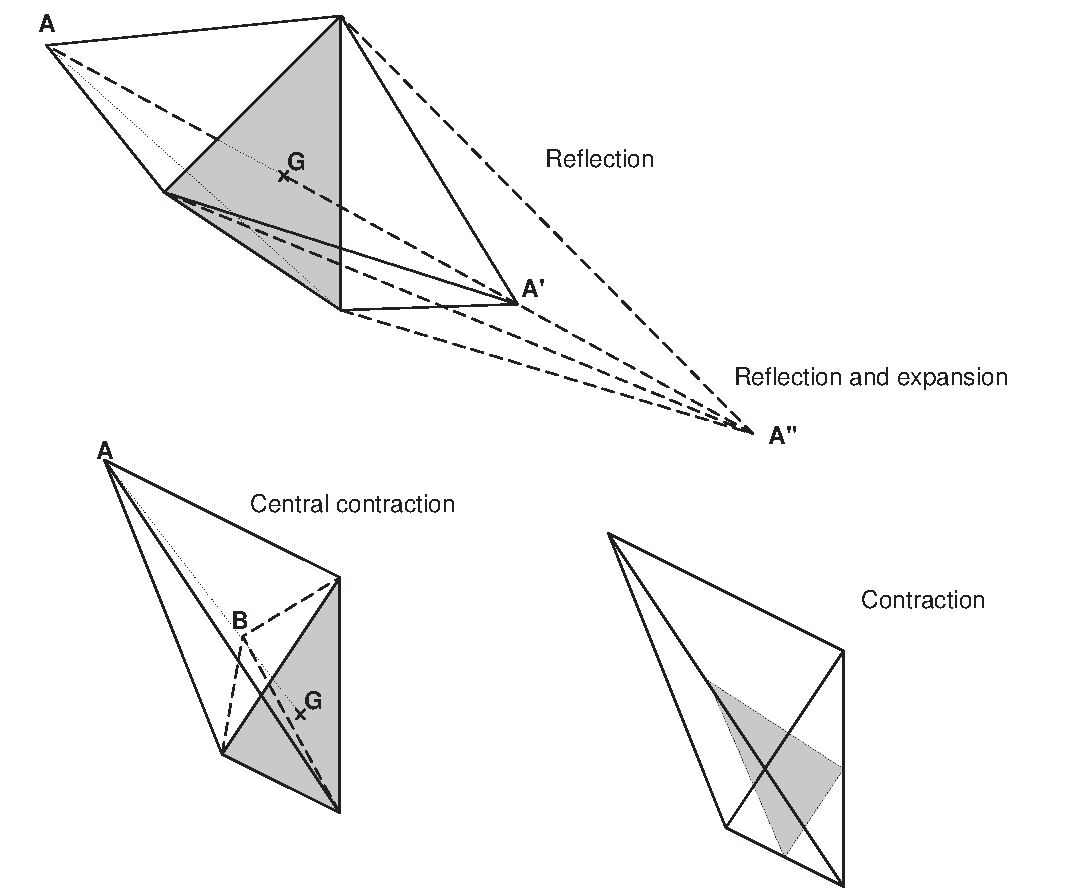
\includegraphics[width=10cm]{Figures/Simplex}
\caption{Operations of the simplex
algorithm}\label{fig:simplexsample}
\end{figure}
Step 6 makes the simplex grow into the direction where the
function is the best so far. Thus, the simplex becomes elongated
in the expected direction of the optimum. Because of its
geometrical shape, the next step is necessarily taken along
another direction, causing an exploration of the regions
surrounding the growth obtained at the preceding step. Over the
iterations, the shape of the simplex adapts itself to narrow
valleys where the hill climbing algorithms notoriously get into
trouble. Steps 9 and 11 ensures the convergence of the algorithm
when the optimum lies inside the simplex. In this mode the simplex
works very much like the golden section search or the bisection
algorithms.

Finding the initial points can be done in several ways. If a good
approximation of the region where the maximum might be located can
be obtained one uses that approximation as a start and generate
$n$ other points by finding the optimum of the function along each
axis. Otherwise, one can generate random points and select $n+1$
points yielding the best values to build the initial simplex. In
all cases, one must make sure that the initial simplex has a
non-vanishing size in all dimensions of the space. Otherwise the
algorithm will not reach the optimum.

\subsection{Simplex algorithm --- General implementation}
The class implementing the simplex algorithm belong to the
hierarchy of the iterative processes discussed in chapter
\ref{ch:iteration}. The method {\texttt evaluateIteration} directly
implements the steps of the algorithm as described above. The
points ${\textbf G}$, ${\textbf A}^{\prime}$, ${\textbf A}^{\prime\prime}$ and
${\textbf B}$ are calculated using the vector operations described in
section \ref{sec:linearalgebra}.

The routine {\texttt initializeIterations} assumes that an initial
value has been provided. It then finds the location of an optimum
of the goal function along each axis of the reference system
starting each time from the supplied initial value, unlike hill
climbing algorithms. Restarting from the initial value is
necessary to avoid creating a simplex with a zero volume. Such
mishaps can arise when the initial value is located on an axis of
symmetry of the goal function.
This can happen quite frequently with {\textsl educated guesses}.

\subsection{Simplex algorithm --- Smalltalk implementation}
\marginpar{Figure \ref{fig:soptimizingclasses} with the box {\textbf
SimplexOptimizer} grayed.} Listing \ref{ls:optimizersimplex} shows
the Smalltalk implementation of the simplex algorithm. The
following code example shows how to invoke the class to find the
minimum of a vector function.

\begin{displaycode}{Smalltalk}
 | fBlock educatedGuess simplex result |
\end{displaycode}
 {\texttt fBlock :=<\textsl the goal function\texttt >}\hfil\break
 {\texttt educatedGuess :=<\textsl a vector in the search space\texttt >}
\begin{displaycode}{Smalltalk}
 simplex := DhbSimplexOptimizer minimizingFunction: fBlock.
 simplex initialValue: educatedGuess.
 result := simplex evaluate
\end{displaycode}
Except for the line creating the instance of the simplex
optimizer, this code example is identical to the example of
Powell's hill climbing algorithm (code example \ref{ex:spowell}).

The class {\texttt DhbSimplexOptimizer} is a subclass of class {\texttt
DhbFunctionOptimizer}. In order to be able to use the iterator
methods efficiently, the worst point of the simplex, ${\textbf A}$, is
held in a separate instance variable {\texttt worstPoint}. As we do
not need to know the function's value $f\left({\textbf A}\right)$, it
is kept as a vector. The remaining points of the simplex are kept
in the instance variable {\texttt bestPoints} of the superclass. Since
this collection is sorted automatically when points are inserted
to it, there is no explicit sorting step.

\begin{listing} Smalltalk implementation of simplex algorithm
\label{ls:optimizersimplex}
$$\halign{ #\hfil&\quad#\hfil\cr {\sl Class}& {\Large\bf DhbSimplexOptimizer}\cr
{\sl Subclass of }&{\tt DhbFunctionOptimizer}\cr\noalign{\vskip 1ex}

{\sl Instance variable names:}&\parbox[t]{4 in}{\tt  worstVector }\cr\noalign{\vskip 1ex}}$$


Class methods
{\parskip 1ex\par\noindent}
{\bf defaultPrecision}
\begin{verbatim}
    ^DhbFloatingPointMachine new defaultNumericalPrecision * 1000

\end{verbatim}



Instance methods
{\parskip 1ex\par\noindent}
{\bf buildInitialSimplex}
\begin{verbatim}
    | projectedFunction finder partialResult |
    projectedFunction := DhbProjectedOneVariableFunction 
                function: functionBlock.
    finder := DhbOneVariableFunctionOptimizer forOptimizer: self.
    finder setFunction: projectedFunction.
    [bestPoints size < (result size + 1)] whileTrue: 
            [projectedFunction
                setArgument: result;
                bumpIndex.
            partialResult := finder
                        reset;
                        evaluate.
            bestPoints add: (optimizingPointClass 
                        vector: (projectedFunction argumentWith: 
                                                        partialResult)
                        function: functionBlock)]

\end{verbatim}
{\bf computeInitialValues}
\begin{verbatim}
    bestPoints 
        add: (optimizingPointClass vector: result function: 
                                                       functionBlock).
    self buildInitialSimplex.
    worstVector := bestPoints removeLast position

\end{verbatim}
{\bf computePrecision}
\begin{verbatim}
    | functionValues bestFunctionValue |
    functionValues := bestPoints collect: [ :each | each value].
    bestFunctionValue := functionValues removeFirst.
    ^functionValues inject: 0
                    into: [ :max :each | ( self precisionOf: ( each - 
   bestFunctionValue) abs relativeTo: bestFunctionValue abs) max: max]

\end{verbatim}
{\bf contract}
\begin{verbatim}
    | bestVector oldVectors |
    bestVector := bestPoints first position.
    oldVectors := OrderedCollection with: worstVector.
    [bestPoints size > 1] whileTrue: [oldVectors add: bestPoints 
                                                 removeLast position].
    oldVectors do: [:each | self contract: each around: bestVector].
    worstVector := bestPoints removeLast position.
    ^self computePrecision

\end{verbatim}
{\bf contract:} {\tt aVector} {\bf around:} {\tt bestVector}
\begin{verbatim}
    bestPoints 
        add: (optimizingPointClass vector: bestVector * 0.5 + 
                                                       (aVector * 0.5)
                function: functionBlock)

\end{verbatim}
{\bf evaluateIteration}
\begin{verbatim}
    | centerOfGravity newPoint nextPoint |
    centerOfGravity := (bestPoints inject: ((worstVector copy)
                        atAllPut: 0;
                        yourself)
                into: [:sum :each | each position + sum]) * (1 / 
                                                     bestPoints size).
    newPoint := optimizingPointClass vector: 2 * centerOfGravity - 
                                                           worstVector
                function: functionBlock.
    (newPoint betterThan: bestPoints first) 
        ifTrue: 
            [nextPoint := optimizingPointClass 
                        vector: newPoint position * 2 - 
                                                       centerOfGravity
                        function: functionBlock.
            (nextPoint betterThan: newPoint) ifTrue: [newPoint := 
                                                           nextPoint]]
        ifFalse: 
            [newPoint := optimizingPointClass 
                        vector: centerOfGravity * 0.666667 + 
                                              (worstVector * 0.333333)
                        function: functionBlock.
            (newPoint betterThan: bestPoints first) ifFalse: [^self 
                                                           contract]].
    worstVector := bestPoints removeLast position.
    bestPoints add: newPoint.
    result := bestPoints first position.
    ^self computePrecision

\end{verbatim}
{\bf printOn:} {\tt aStream}
\begin{verbatim}
    super printOn: aStream.
    aStream cr. 
    worstVector printOn: aStream.

\end{verbatim}


\end{listing}

\section{Genetic algorithm}
All optimizing algorithm discussed so far have one common flaw:
they all terminate when a local optimum is encountered. In most
problems, however, one wants to find the absolute optimum of the
function. This is especially true if the goal function represents
some economical merit.

\noindent One academic example is the maximization of the function
\begin{equation}
\label{eq:geneticCase}
  f\left({\textbf x}\right)={ \sin^2\left|{\textbf x}\right| \over\left|{\textbf
  x}\right|^2}.
\end{equation}
This function has an absolute maximum at ${\textbf x}=0$, but all
algorithms discussed so far will end up inside a ring
corresponding to $\left|{\textbf x}\right|=n\pi/2$ where $n$ is any
positive odd integer.

In 1975 John Holland introduced a new type of algorithm --- dubbed
genetic algorithm --- because it tries to mimic the evolutionary
process identified as the cause for the diversity of living
species by Charles Darwin. In a genetic algorithm the elements of
the search space are considered as the chromosomes of individuals;
the goal function is considered as the measure of the fitness of
the individual to adapt itself to its
environment\cite{BerLin}\cite{Koza}. The iterations are aping (pun
intended) the Darwinian principle of survival and reproduction. At
each iteration, the fittest individuals survive and reproduce
themselves. To bring some variability to the algorithm mutation
and crossover of chromosomes are taken into account.

Mutation occurs when one gene of a chromosome is altered at
reproduction time. Crossover occurs when two chromosomes break
themselves and recombine with the piece coming from the other
chromosome. These processes are illustrated on figure
\ref{fig:crossover}.
\begin{figure}
\centering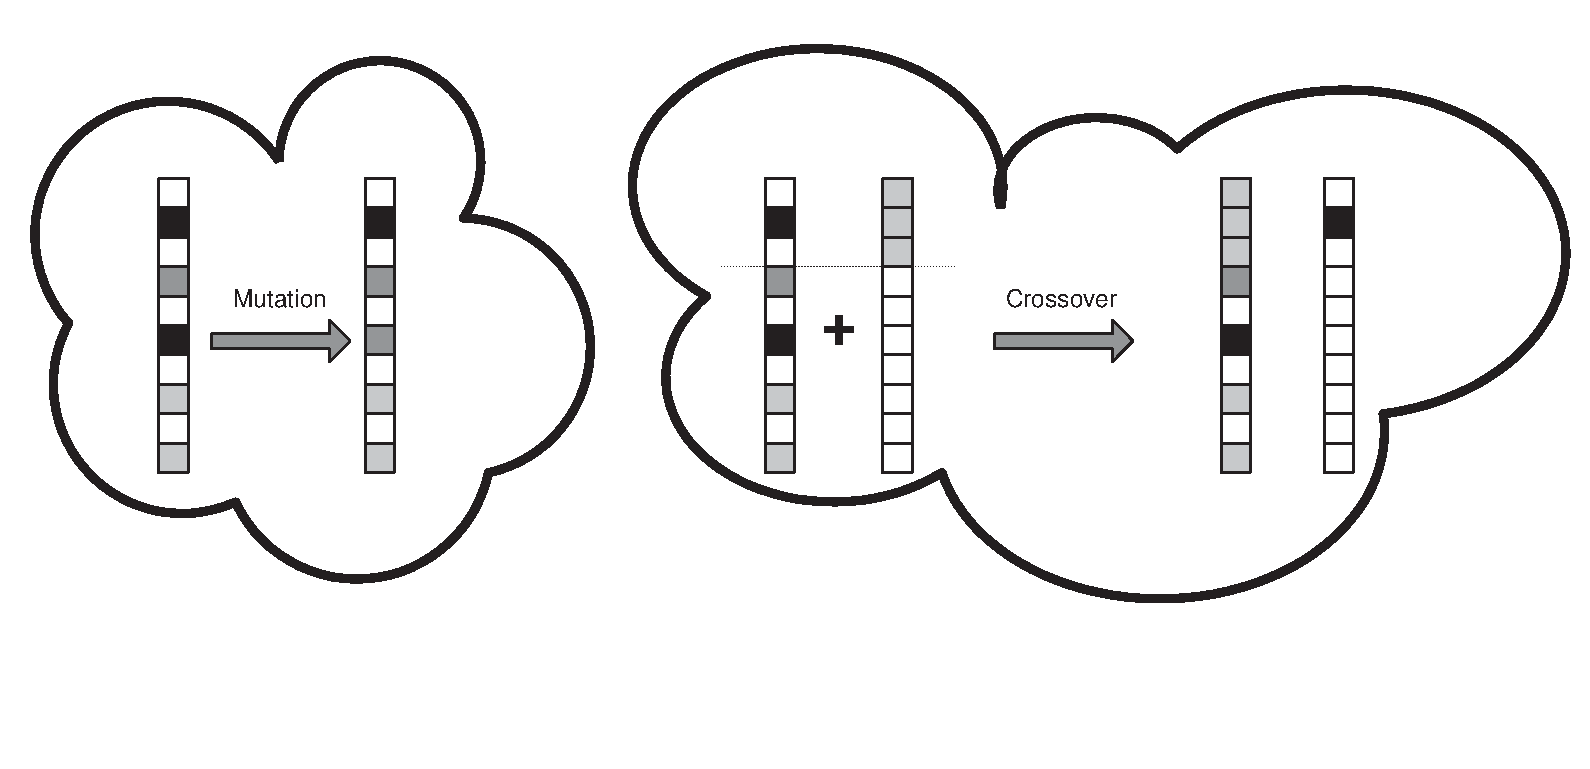
\includegraphics[width=11cm]{Figures/Crossover}
\caption{Mutation and crossover reproduction of
chromosomes}\label{fig:crossover}
\end{figure}
The point where the chromosomes are breaking is called the
crossover point. Which individual survives and reproduces itself,
when and where mutation occurs and when and where a crossover
happens is determined randomly. This is precisely the random
nature of the algorithm which gives it the ability to jump out of
a local optimum to look further for the absolute optimum.

\rubrique{Mapping the search space on chromosomes} To be able to
implement a genetic algorithm one must establish how to represent
the genes of a chromosome. At the smallest level the genes could
be the bits of the structure representing the chromosome. If the
search space of the goal function do cover the domain generated by
all possible permutations of the bits, this is a good approach.
However, this is not always a practical solution since some bit
combinations may be forbidden by the structure. For example, some
of the combinations of a 64 bit word do not correspond to a valid
floating point number.

In the case of the optimization of a vector function, the simplest
choice is to take the components of the vector as the genes.
Genetic algorithms are used quite often to adjust the parameters
of a neural network \cite{BerLin}. In this case, the chromosomes
are the coefficients of each neuron. Chromosomes can even be
computer subprograms in the case of genetic programming
\cite{Koza}. In this latter case, each individual is a computer
program trying to solve a given problem.

Figure \ref{fig:geneticFlow} shows a flow diagram of a general
genetic algorithm.
\begin{figure}
\centering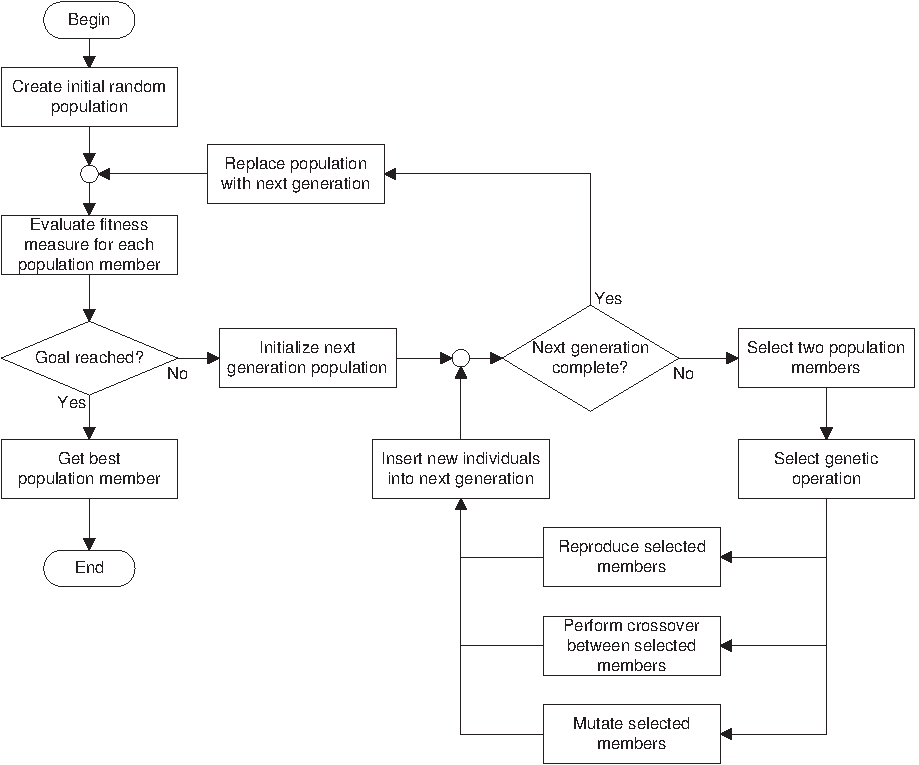
\includegraphics[width=10cm]{Figures/GeneticFlow}
\caption{General purpose genetic algorithm}\label{fig:geneticFlow}
\end{figure}
The reproduction of the individual is taken literally: a copy of
the reproducing individual is copied into the next generation. The
important feature of a generic algorithm is that the building of
the next generation is a random process. To ensure the survival of
the fittest, the selection of the parents of the individuals of
the next generation is performed at random with uneven
probability: the fittest individuals have a larger probability of
being selected than the others. Mutation enables the algorithm to
create individuals having genes corresponding to unexplored
regions of the search space. Most of the times such mutants will
be discarded at the next iteration; but, in some cases, a mutation
may uncover a better candidate. In the case of the function of
equation \ref{eq:geneticCase}, this would correspond to jumping
from one ring to another ring closer to the function's maximum.
Finally the crossover operation mixes good genes in the hope of
building a better individual out of the properties of good
inidividuals. Like mutation the crossover operation gives a
stochastic behavior to the algorithm enabling it to explore
uncharted regions of the search space.

\note{Because of its stochastic nature a genetic algorithm is the
algorithm of choice when the goal function is expressed on
integers.}

\subsection{Genetic algorithm --- General implementation}
\label{sec:gengenetic} The left hand side of the diagram of figure
\ref{fig:geneticFlow} is quite similar to the flow diagram of an
iterative process (\cf figure \ref{fig:itercoarse} in chapter
\ref{ch:iteration}). Thus, the class implementing the genetic
algorithm is a subclass of the iterative process class discussed
in chapter \ref{ch:iteration}.

The {\textsl genetic} nature of the algorithm is located in the right
hand side of the diagram of figure \ref{fig:geneticFlow}. As we
have mentioned before the implementation of the chromosomes is
highly problem dependent. All operations located in the top
portion of the mentioned area can be expressed in generic terms
without any knowledge of the chromosomic implementation. to handle
the lower part of the right hand side of the diagram of figure
\ref{fig:geneticFlow}, we shall implement a new object, the
chromosome manager.

One should also notice that the value of the function is not
needed when the next generation is build. Thus, the chromosome
manager does not need to have any knowledge of the goal function.
The goal function comes into play when transfering the next
generation to the {\textsl mature} population, that is, the population
used for reproduction at the next iteration . At the maturity
stage, the value of the goal function is needed to identify the
fittest individuals. In our implementation, the next generation is
maintained by the chromosome manager whereas the population of
mature individuals is maintained by the object in charge of the
genetic algorithm which has the knowledge of the goal function.

\noindent The chromosome manager has the following instance
variables:
\begin{description}
  \item[\texttt populationSize] contains the size of the population;
  one should pick up a large enough number to be able to cover the
  search space efficiently: the larger the dimension of the space
  search space, the larger must be the population size;
  \item[\texttt rateOfMutation] contains the probability of having a
  mutation while reproducing;
  \item[\texttt rateOfCrossover] contains the probability of having a
  crossover while reproducing.
\end{description}
All of these variables have getter and setter accessor methods. In
addition a convenience instance creation method is supplied to
create a chromosome manager with given values for all three
instance variables. The chromosome manager implements the
following methods:
\begin{description}
  \item[\texttt isFullyPopulated] to signal that a sufficient number of individuals
  has been generated into the population;
  \item[\texttt process] to process a pair of individuals; this method
  does the selection of the genetic operation and applies it;
  individuals are processed by pair to always have a possibility
  of crossover;
  \item[\texttt randomnizePopulation] to generate a random population;
  \item[\texttt reset] to create an empty population for the next
  generation.
\end{description}
Finally the chromosome manager must also implement methods
performing each of the genetic operations: reproduction, mutation
and crossover. The Smalltalk implementation supplies methods that
returns a new individual.

The genetic optimizer is the object implementing the genetic
algorithm proper. It is a subclass of the iterative process class
described in chapter \ref{sec:iterrel}. In addition to the
handling of the iterations the genetic optimizer implements the
steps of the algorithm drawn on the top part of the right hand
side of the diagram of figure \ref{fig:geneticFlow}. It has one
instance variable containing the chromosome manager with which it
will interact. The instance creation method take three arguments:
the function to optimize, the optimizing strategy and the
chromosome manager.

The method {\texttt initializeIteration} asks the chromosome manager
to supply a random population. The method {\texttt evaluateIteration}
performs the loop of the right hand side of the diagram of figure
\ref{fig:geneticFlow}. It selects a pair of parents on which the
chromosome manager performs the genetic operation.

Selecting the genetic operation is performed with a random
generator. The values of the goal function are used as weights.
Let $f\left(p_i\right)$ be the value of the goal function for
individual $p_i$ and let $p_b$ and $p_w$ be respectively the
fittest and the lest fit individual found so far ($b$ stands for
best and $w$ stands for worst). One first computes the
unnormalized probability:
\begin{equation}
  \tilde{P}_i={\displaystyle f\left(p_i\right) - f\left(p_w\right)
  \over\displaystyle f\left(p_b\right) - f\left(p_w\right)}.
\end{equation}
This definition ensures that $\tilde{P}_i$ is always comprised
between 0 and 1 for any goal function. Then we can use the
discrete probability
\begin{equation}
\label{eq:geneticprob}
  P_i={\displaystyle  1
  \over\displaystyle \sum\tilde{P}_i} \tilde{P}_i.
\end{equation}
The sum in equation \ref{eq:geneticprob} is taken over the entire
population. An attentive reader will notice than this definition
assigns a zero probability of selecting the worst individuals.
This gives a slight bias to our implementation compared to the
original algorithm. This is can be easily compensated by taking a
sufficiently large population. The method {\texttt randomScale}
calculates the $P_i$ of equation \ref{eq:geneticprob} and returns
an array containing the integrated sums:
\begin{equation}
  R_i=\sum_{k=0}^i P_i.
\end{equation}
The array $R_i$ is used to generate a random index to select
individuals for reproduction.

\noindent The transfer between the next generation and the mature
population is performed by the method {\texttt collectPoints}.

In the general case, there is no possibility to decide when the
terminate the algorithm. In practice, it is possible that the
population stays stable for quite a while until suddenly a new
individual is found to be better than the rest. Therefore a
criteria based on the stability of the first best points is likely
to be beat the purpose of the algorithm, namely to jump out of a
local optimum. Some problems can define a threshold at which the
goal function is considered sufficiently good. In this case, the
algorithm can be stopped as soon as the value of the goal function
for the fittest individual becomes better than that threshold. In
the general case, however, the implementation of the genetic
algorithm simply returns a constant pseudo precision
--- set to one --- and runs until the maximum number of iterations
becomes exhausted.

\subsection{Genetic algorithm --- Smalltalk implementation}
\marginpar{Figure \ref{fig:soptimizingclasses} with the boxes {\textbf
GeneticOptimizer}, {\textbf ChromosomeManager} and {\textbf
VectorChromosomeManager} grayed.} Listing \ref{ls:chromosome}
shows the code of an abstract chromosome manager in Smalltalk and
of a concrete implementation for vector chromosomes. The class
{\texttt DhbChromosomeManager} has one instance variable in addition
to the variables listed in section \ref{sec:gengenetic}: {\texttt
population}. This variable is an instance of an {\texttt
OrderedCollection} containing the individuals of the next
generation being prepared.

The class {\texttt DhbVectorChromosomeManager} is a sublcass of class
{\texttt DhbChromosomeManager} implementing vector chromosomes. It has
two instance variables
\begin{description}
  \item[\texttt origin] a vector containing the minimum possible
  values of the generated vectors;
  \item[\texttt range] a vector containing the range of the generated
  vectors.
\end{description}
In other words {\texttt origin} and {\texttt range} are delimiting an
hypercube defining the search space.

\begin{listing} Smalltalk chromosome: abstract and concrete \label{ls:chromosome}
$$\halign{ #\hfil&\quad#\hfil\cr {\sl Class}& {\Large\bf DhbChromosomeManager}\cr
{\sl Subclass of }&{\tt Object}\cr\noalign{\vskip 1ex}

{\sl Instance variable names:}&\parbox[t]{4 in}{\tt  population populationSize rateOfMutation rateOfCrossover }\cr\noalign{\vskip 1ex}}$$


Class methods
{\parskip 1ex\par\noindent}
{\bf new:} {\tt anInteger} {\bf mutation:} {\tt aNumber1} {\bf crossover:} {\tt aNumber2}
\begin{verbatim}
    ^ self new populationSize: anInteger; rateOfMutation: aNumber1; 
                                   rateOfCrossover: aNumber2; yourself
\end{verbatim}

Instance methods
{\parskip 1ex\par\noindent}
{\bf clone:} {\tt aChromosome}
\begin{verbatim}
    ^ aChromosome copy
\end{verbatim}
{\bf crossover:} {\tt aChromosome1} {\bf and:} {\tt aChromosome2}
\begin{verbatim}
    ^ self subclassResponsibility
\end{verbatim}
{\bf isFullyPopulated}
\begin{verbatim}
    ^ population size >= populationSize 
\end{verbatim}
{\bf mutate:} {\tt aChromosome}
\begin{verbatim}
    ^ self subclassResponsibility
\end{verbatim}
{\bf population}
\begin{verbatim}
    ^ population
\end{verbatim}
{\bf populationSize:} {\tt anInteger}
\begin{verbatim}
    populationSize := anInteger.
\end{verbatim}
{\bf process:} {\tt aChromosome1} {\bf and:} {\tt aChromosome2}
\begin{verbatim}
    | roll |
    roll := Number random.
    roll < rateOfCrossover 
        ifTrue: [population addAll: (self crossover: aChromosome1 
                                                   and: aChromosome2)]
        ifFalse: 
            [roll < (rateOfCrossover + rateOfMutation) 
                ifTrue: 
                    [population
                        add: (self mutate: aChromosome1);
                        add: (self mutate: aChromosome2)]
                ifFalse: 
                    [population
                        add: (self clone: aChromosome1);
                        add: (self clone: aChromosome2)]]
\end{verbatim}
{\bf randomnizePopulation}
\begin{verbatim}
    self reset.
    [ self isFullyPopulated] whileFalse: [ population add: self 
                                                    randomChromosome].
\end{verbatim}
{\bf rateOfCrossover:} {\tt aNumber}
\begin{verbatim}
    (aNumber between: 0 and: 1) 
        ifFalse: [self error: 'Illegal rate of cross-over'].
    rateOfCrossover := aNumber
\end{verbatim}
{\bf rateOfMutation:} {\tt aNumber}
\begin{verbatim}
    (aNumber between: 0 and: 1) 
        ifFalse: [self error: 'Illegal rate of mutation'].
    rateOfMutation := aNumber
\end{verbatim}
{\bf reset}
\begin{verbatim}
    population := OrderedCollection new: populationSize.
\end{verbatim}


$$\halign{ #\hfil&\quad#\hfil\cr {\sl Class}& {\Large\bf DhbVectorChromosomeManager}\cr
{\sl Subclass of }&{\tt DhbChromosomeManager}\cr\noalign{\vskip 1ex}

{\sl Instance variable names:}&\parbox[t]{4 in}{\tt  origin range }\cr\noalign{\vskip 1ex}}$$

Instance methods
{\parskip 1ex\par\noindent}
{\bf crossover:} {\tt aChromosome1} {\bf and:} {\tt aChromosome2}
\begin{verbatim}
    | index new1 new2|
    index := (aChromosome1 size - 1) random + 2.
    new1 := self clone: aChromosome1.
    new1 replaceFrom: index to: new1 size with: aChromosome2 
                                                    startingAt: index.
    new2 := self clone: aChromosome2.
    new2 replaceFrom: index to: new2 size with: aChromosome1 
                                                    startingAt: index.
    ^  Array with: new1 with: new2

\end{verbatim}
{\bf mutate:} {\tt aVector}
\begin{verbatim}
    | index |
    index := aVector size random + 1.
    ^  aVector copy
            at: index put: (self randomComponent: index);
            yourself
\end{verbatim}
{\bf origin:} {\tt aVector}
\begin{verbatim}
    origin := aVector.
\end{verbatim}
{\bf randomChromosome}
\begin{verbatim}
    ^ ((1 to: origin size) collect: [ :n | self randomComponent: n]) 
                                                              asVector
\end{verbatim}
{\bf randomComponent:} {\tt anInteger}
\begin{verbatim}
    ^ (range at: anInteger) random + (origin at: anInteger)
\end{verbatim}
{\bf range:} {\tt aVector}
\begin{verbatim}
    range := aVector.
\end{verbatim}


\end{listing}
Listing \ref{ls:optimizerabsgen} shows how the genetic optimizer
is implemented in Smalltalk. The following code example shows how
to use a genetic optimizer to find the maximum of a vector
function.

\begin{displaycode}{Smalltalk}
    | fBlock optimizer manager origin range result |
\end{displaycode}
 {\texttt fBlock :=<\textsl the goal function\texttt >}\hfil\break
 {\texttt origin :=<\textsl a vector containing the minimum expected value of the component\texttt >}\hfil\break
 {\texttt range :=<\textsl a vector containing the expected range of the component\texttt >}\hfil\break
\begin{displaycode}{Smalltalk}
    optimizer := DhbGeneticOptimizer maximizingFunction: fBlock.
    manager := DhbVectorChromosomeManager new: 100 mutation: 0.1 crossover: 0.1.
    manager origin: origin; range: range.
    optimizer chromosomeManager: manager.
    result := optimizer evaluate
\end{displaycode}
After establishing the goal function and the search space, an
instance of the genetic optimizer is created. The next line
creates an instance of a vector chromosome manager for a
population of 100 individuals (sufficient for a 2-3 dimensional
space) and rates of mutation and crossover equal to $10\%$. The
next line defines the search space into the chromosome manager.
The final line performs the genetic search and returns the result.

In Smalltalk the population of the next generation is maintained
in the instance variable {\texttt population}. Each time a next
generation has been established, it is transferred into a
collection of best points by the method {\texttt collectPoints}. Each
element of the collection {\texttt bestPoints} is an instance of an
subclass of {\texttt OptimizingPoint}. The exact type of the class is
determined by the search strategy. Since best points are sorted
automatically, the result is always the position of the first
element of  {\texttt bestPoints}.

\begin{listing} Smalltalk implementation of genetic algorithm \label{ls:optimizerabsgen}
$$\halign{ #\hfil&\quad#\hfil\cr {\sl Class}& {\Large\bf DhbGeneticOptimizer}\cr
{\sl Subclass of }&{\tt DhbFunctionOptimizer}\cr\noalign{\vskip 1ex}

{\sl Instance variable names:}&\parbox[t]{4 in}{\tt  chromosomeManager }\cr\noalign{\vskip 1ex}}$$


Class methods
{\parskip 1ex\par\noindent}
{\bf defaultMaximumIterations}
\begin{verbatim}
    ^ 500
\end{verbatim}
{\bf defaultPrecision}
\begin{verbatim}
    ^ 0
\end{verbatim}



Instance methods
{\parskip 1ex\par\noindent}
{\bf chromosomeManager:} {\tt aChromosomeManager}
\begin{verbatim}
    chromosomeManager := aChromosomeManager.
    ^ self
\end{verbatim}
{\bf collectPoints}
\begin{verbatim}
    | bestPoint |
    bestPoints notEmpty
        ifTrue: [ bestPoint := bestPoints removeFirst].
    bestPoints removeAll: bestPoints asArray.
    chromosomeManager population do: [:each | self addPointAt: each].
    bestPoint notNil
        ifTrue: [ bestPoints add: bestPoint].
    result := bestPoints first position.

\end{verbatim}
{\bf computePrecision}
\begin{verbatim}
    ^ 1
\end{verbatim}
{\bf evaluateIteration}
\begin{verbatim}
    | randomScale |
    randomScale := self randomScale.
    chromosomeManager reset.
    [ chromosomeManager isFullyPopulated ]
        whileFalse: [ self processRandomParents: randomScale ].
    self collectPoints.
    ^ self computePrecision
\end{verbatim}
{\bf initializeIterations}
\begin{verbatim}
    chromosomeManager randomnizePopulation.
    self collectPoints
\end{verbatim}
{\bf processRandomParents:} {\tt aNumberArray}
\begin{verbatim}
    chromosomeManager process: (bestPoints at: (self randomIndex: 
                                               aNumberArray)) position
                        and:  (bestPoints at: (self randomIndex: 
                                              aNumberArray)) position.
\end{verbatim}
{\bf randomIndex:} {\tt aNumberArray}
\begin{verbatim}
    | x n |
    x := Number random.
    n := 1.
    aNumberArray do: 
        [ :each |
          x < each
            ifTrue: [ ^n ].
          n := n + 1.
        ].
    ^ aNumberArray size  
\end{verbatim}
{\bf randomScale}
\begin{verbatim}
    | norm fBest fWorst answer|
    fBest := bestPoints first value.
    fWorst := bestPoints last value.
    norm := 1 / (fBest - fWorst).
    answer := bestPoints collect: [ :each | (each value - fWorst) * 
                                                                norm ].
    norm := 1 / ( answer inject: 0 into: [ :sum :each | each + sum ]).
    fBest := 0.
    ^ answer collect: [ :each | fBest := each * norm + fBest. fBest ]
\end{verbatim}


\end{listing}


\section{Multiple strategy approach}
\label{sec:multistrategy} As we have seen most of the optimizing
algorithms described so far have some limitation:
\begin{itemize}
  \item Hill climbing algorithms may get into trouble far from the
  optimum and may get caught into a local optimum. This is exemplified in figure \ref{fig:hillvsrandom}.
  \item The simplex algorithm may get caught into a local optimum
  and does not converge well near the optimum.
  \item Genetic algorithms do not have a clear convergence
  criteria.
\end{itemize}
\begin{figure}
\centering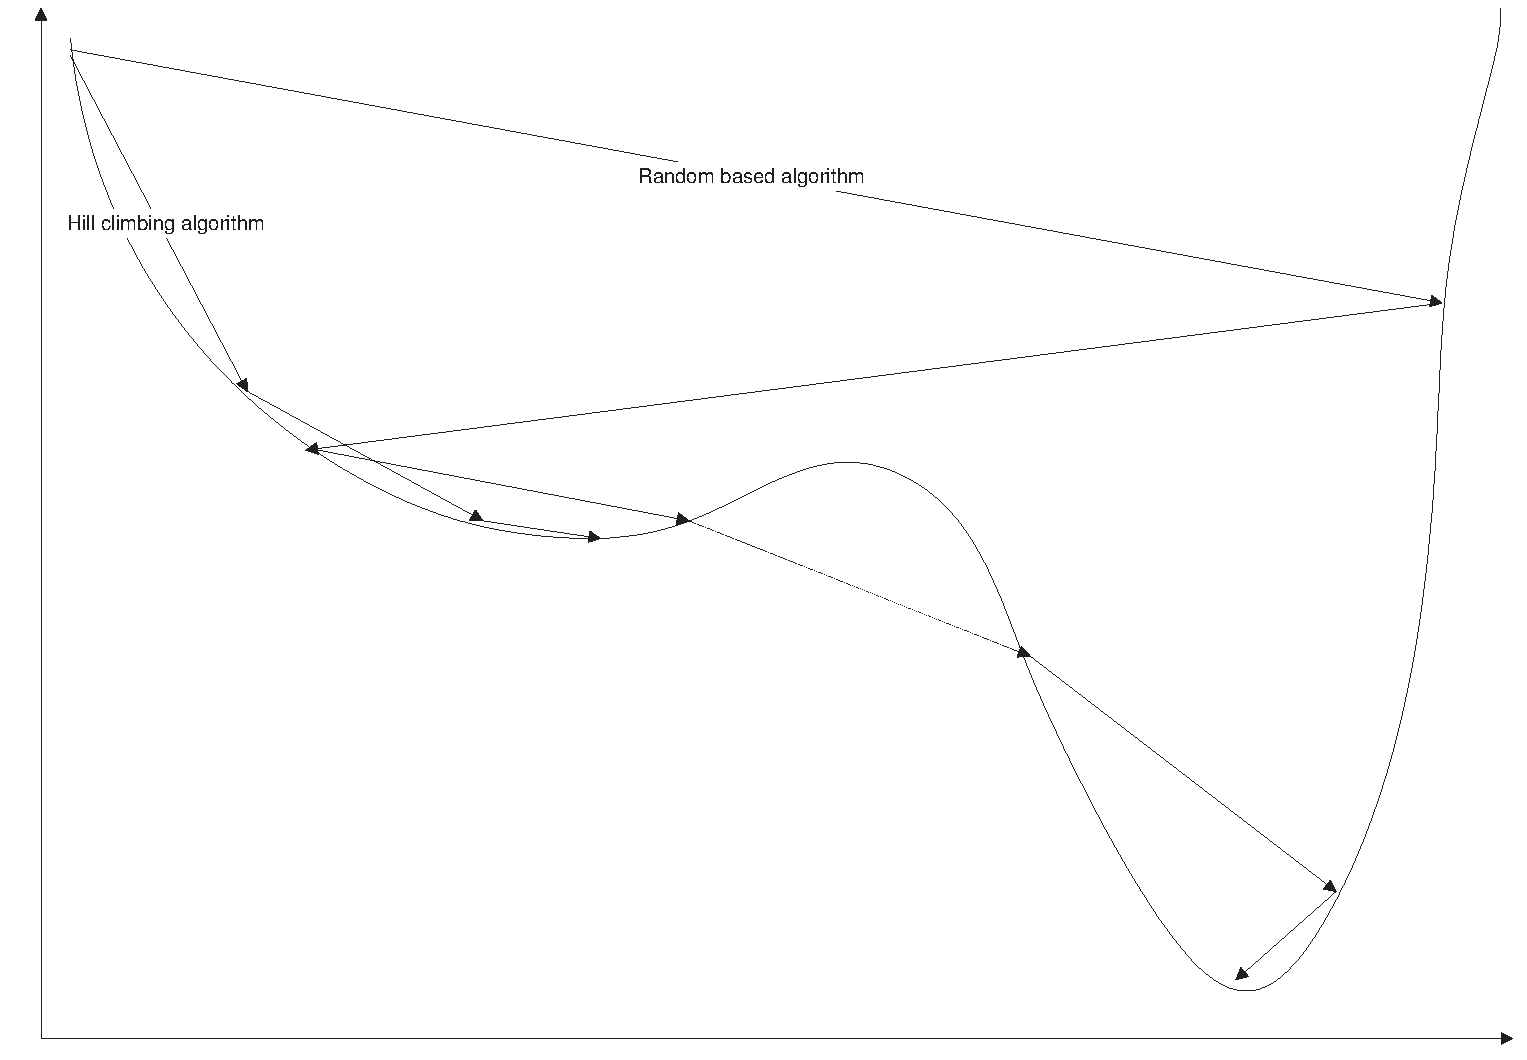
\includegraphics[width=12cm]{Figures/OptimizingComparisonvsd}
\caption{Compared behavior of hill climbing and random based algorithms.}\label{fig:hillvsrandom}
\end{figure}
After reading the above summary of the pro and cons of each
algorithm, the reader may have already come to the conclusion that
mixing the three algorithms together can make a very efficient
strategy to find the optimum of a wide variety of functions.

One can start with a genetic optimizer for a sufficient number of
iterations. This should ensure that the best points found at the
end of the search does not lie too far from the absolute optimum.
Then, one can use the simplex algorithm to get rapidly near the
optimum. The final location of the optimum is obtained using a
hill climbing optimizer.

\subsection{Multiple strategy approach --- General implementation}
This multiple strategy approach, inspired from the program MINUIT,
has been adapted to the use of the algorithms discussed here. The
class {\texttt MultiVariableGeneralOptimizer} combines the three
algorithms: genetic, simplex and hill climbing, in this order. We
could have make it a subclass of {\texttt Object}, but we decided to
reuse all the management provided by the abstract optimizer class
discussed in section \ref{sec:goptonedim}. Therefore, our general
purpose optimizer is a subclass of the abstract optimizer class
although it does not really uses the framework of an iterative
process. We only need one additional instance variable: the range
used to construct the hypercube search space for the vector
genetic chromosome manager. A corresponding setting method is
provided: {\texttt setRange}.

The method {\texttt initializeIterations} performs search using the
genetic algorithm as an option and, then, the simplex algorithm.
Since the genetic algorithm require a great deal of function
evaluate --- due to its stochastic nature --- it is a good idea to
give the user the choice of by-passing the use of the genetic
algorithm. If no range has been defined, only the simplex
algorithm is used from the supplied initial value. Otherwise a
search is made with the genetic algorithm using the initial value
and the range to define the search space. Then the simplex
algorithm is started from the best point found by the genetic
algorithm. The precision for the simplex search is set to the
square root of the precision for the final search. Less precision
is required for this step because the final search will give a
better precision.

The method {\texttt evaluateIteration} performs the hill climbing
algorithm and returns it precision. As the desired precision of
the hill climbing algorithm is set to that of the general purpose
optimizer. As a consequence, there will only be a single
iteration.

Listing \ref{ls:optimizergeneral} shows the implementation in
Smalltalk. At this point we shall abstain from
commenting the code as the reader should have no more need for
such thing$\ldots$ Hopefully!

\marginpar{Figure \ref{fig:soptimizingclasses} with the box {\textbf
MultiVariableGeneralOptimizer} grayed.}
\begin{listing} Smalltalk
implementation of a general optimizer \label{ls:optimizergeneral}
$$\halign{ #\hfil&\quad#\hfil\cr {\sl Class}& {\Large\bf DhbMultiVariableGeneralOptimizer}\cr
{\sl Subclass of }&{\tt DhbFunctionOptimizer}\cr\noalign{\vskip 1ex}
}$$


Instance methods
{\parskip 1ex\par\noindent}
{\bf computeInitialValues}
\begin{verbatim}
    self range notNil
        ifTrue: [ self performGeneticOptimization].
    self performSimplexOptimization.
\end{verbatim}
{\bf evaluateIteration}
\begin{verbatim}
    | optimizer |
    optimizer := DhbHillClimbingOptimizer forOptimizer: self.
    optimizer desiredPrecision: desiredPrecision;
              maximumIterations: maximumIterations.
    result := optimizer evaluate.
    ^ optimizer precision
\end{verbatim}
{\bf origin}
\begin{verbatim}
    ^ result
\end{verbatim}
{\bf origin:} {\tt anArrayOrVector}
\begin{verbatim}
    result := anArrayOrVector.
\end{verbatim}
{\bf performGeneticOptimization}
\begin{verbatim}
    | optimizer manager |
    optimizer := DhbGeneticOptimizer forOptimizer: functionBlock.
    manager := DhbVectorChromosomeManager new: 100 mutation: 0.1 
                                                       crossover: 0.1.
    manager origin: self origin asVector; range: self range asVector.
    optimizer chromosomeManager: manager.
    result := optimizer evaluate.
\end{verbatim}
{\bf performSimplexOptimization}
\begin{verbatim}
    | optimizer manager |
    optimizer := DhbSimplexOptimizer forOptimizer: self.
    optimizer desiredPrecision: desiredPrecision sqrt;
              maximumIterations: maximumIterations;
              initialValue: result asVector.
    result := optimizer evaluate.
\end{verbatim}
{\bf range}
\begin{verbatim}
    ^ self bestPoints
\end{verbatim}
{\bf range:} {\tt anArrayOrVector}
\begin{verbatim}
    bestPoints := anArrayOrVector.
\end{verbatim}


\end{listing}

%\ifx\wholebook\relax\else\end{document}\fi
